% !TEX root = ../../技术文档.tex
\section{CPU设计}

\subsection{CPU微架构}

CPU采用RV32IM、Zicsr与Zifencei指令集\cite{riscv-unpriv-20260120}，支持机器模式异常处理，承担裸机程序执行、外设控制、NPU任务配置和检测后处理。
指令长度固定为32\,bit，整数寄存器与地址宽度均为32\,bit。
六级顺序流水线支持单发射和双发射配置。双发射时，每周期最多发射两条相邻指令，程序顺序靠前的指令使用A槽，靠后的指令使用B槽；B槽只有在A槽可接纳时才发射。
顶层参数\texttt{DUAL\_ISSUE}取0选择单发射，取1选择双发射，并向内核传递为\texttt{SUPPORT\_DUAL\_ISSUE}。
该参数在综合时确定硬件结构，不通过软件在运行时切换。单发射配置不生成第二执行单元，寄存器堆使用2读1写接口；双发射配置使用两条执行通路和4读2写接口。
两种配置共用六级流水边界、指令集、异常接口和存储协议。本节结构图以双发射配置展示完整数据通路，单发射配置每周期仅接纳A槽指令。
程序通过物理地址访问存储空间，启动入口映射到\texttt{0x0000\,0000}处的Boot ROM。

取指前端、双候选译码、寄存器堆及前递网络向两条执行通路提供指令和操作数。
两路整数运算单元分别处理A、B槽指令，LSU和乘法器各由一个实例共享，除法与CSR仅由A槽使用。
I-Cache与D-Cache分别服务取指和数据访问，本地ROM、SRAM及不可缓存设备由地址路由选择访问路径。
独立TCM配置直接接入片上存储，不实例化I/D Cache及DDR控制器；缓存配置通过I/D Cache访问DDR，两类性能结果分别统计。
CPU主要配置见表\ref{tbl:cpu-configuration}。

人脸检测应用采用50\,MHz单发射控制配置，程序、数据和栈位于32\,KiB片上SRAM，CPU通过不可缓存访问路径读取DDR中的检测输出。
该配置设置\texttt{MINIMAL\_CONTROL\_CPU=1}和\texttt{CACHE\_ENABLE=0}，保留整数乘除法、机器模式CSR和异常处理。
相对于通用配置，分支预测、BHT与RAS使能置零，Load/MUL及提前MUL结果旁路置零；BTB/BHT规模参数由512项缩为2项，但预测模块不参与该配置的取指。相关指令按结果就绪条件推进。
应用由CPU处理控制和后处理任务，NPU执行计算图，片上SRAM承担程序与数据访问。整机以功能和时序验收为优先，采用与资源、时钟跨域及布线约束配套的50\,MHz工作点，计算域Slow角建立裕量为+2.287\,ns。
本节按通用配置介绍CPU各模块；独立CPU的100\,MHz CoreMark测试采用各自构建，结果不代入该应用配置。

\begin{reporttable}
\begin{longtable}{@{}p{0.25\linewidth}p{0.70\linewidth}@{}}
\caption{CPU主要配置}\label{tbl:cpu-configuration}\\
\toprule
项目 & 配置 \\
\midrule
\endfirsthead
\caption[]{CPU主要配置（续）}\\
\toprule
项目 & 配置 \\
\midrule
\endhead
\bottomrule
\endfoot
指令与模式 & RV32IM、Zicsr、Zifencei，M-mode \\
流水线 & IF1、IF2、ID、E1、E2、WB；顺序双发射，可配置为单发射 \\
通用寄存器 & 32个32\,bit寄存器；单发射2读1写，双发射4读2写，\texttt{x0}恒为零 \\
取指接口 & 32\,bit地址、64\,bit返回数据，8\,B对齐取指包 \\
数据接口 & 32\,bit地址与数据、4\,bit写字节使能 \\
指令FIFO & 六条指令容量，每项119\,bit载荷，双队首缓存，可跨包配对 \\
分支预测 & 512项BTB、512项两位BHT、4项RAS \\
执行资源 & 两路ALU、共享LSU和MUL、A槽专用DIV和CSR \\
L1-Cache & I/D各16\,KiB，两路组相联、256组、32\,B行；D-Cache写回、写分配 \\
结果前递 & 两条通路的E1、E2及WB；按结果类型和就绪条件选择 \\
\end{longtable}
\end{reporttable}

图\ref{fig:cpu-pipeline}给出六级流水线的模块划分、两条执行通路与共享资源，窄寄存器符号及带内侧竖线的状态框标出寄存位置。ID级包含寄存器读取、相关性检查、前递选择和组合ALU运算，
整数结果在ID/E1边界保存；E1使用已寄存的分支操作数解析通用分支，保持整数结果并发出访存请求。
因此，六级划分不意味着全部算术组合逻辑都位于E1，ID的时序路径同时包含操作数选择与ALU计算。
图中实线表示数据通路，虚线表示控制关系，浅色分区区分流水级或功能区域；寄存状态用窄条或带内侧竖线的方框表示，此约定同样用于后续结构图。

\begin{figure}[!htbp]
\centering
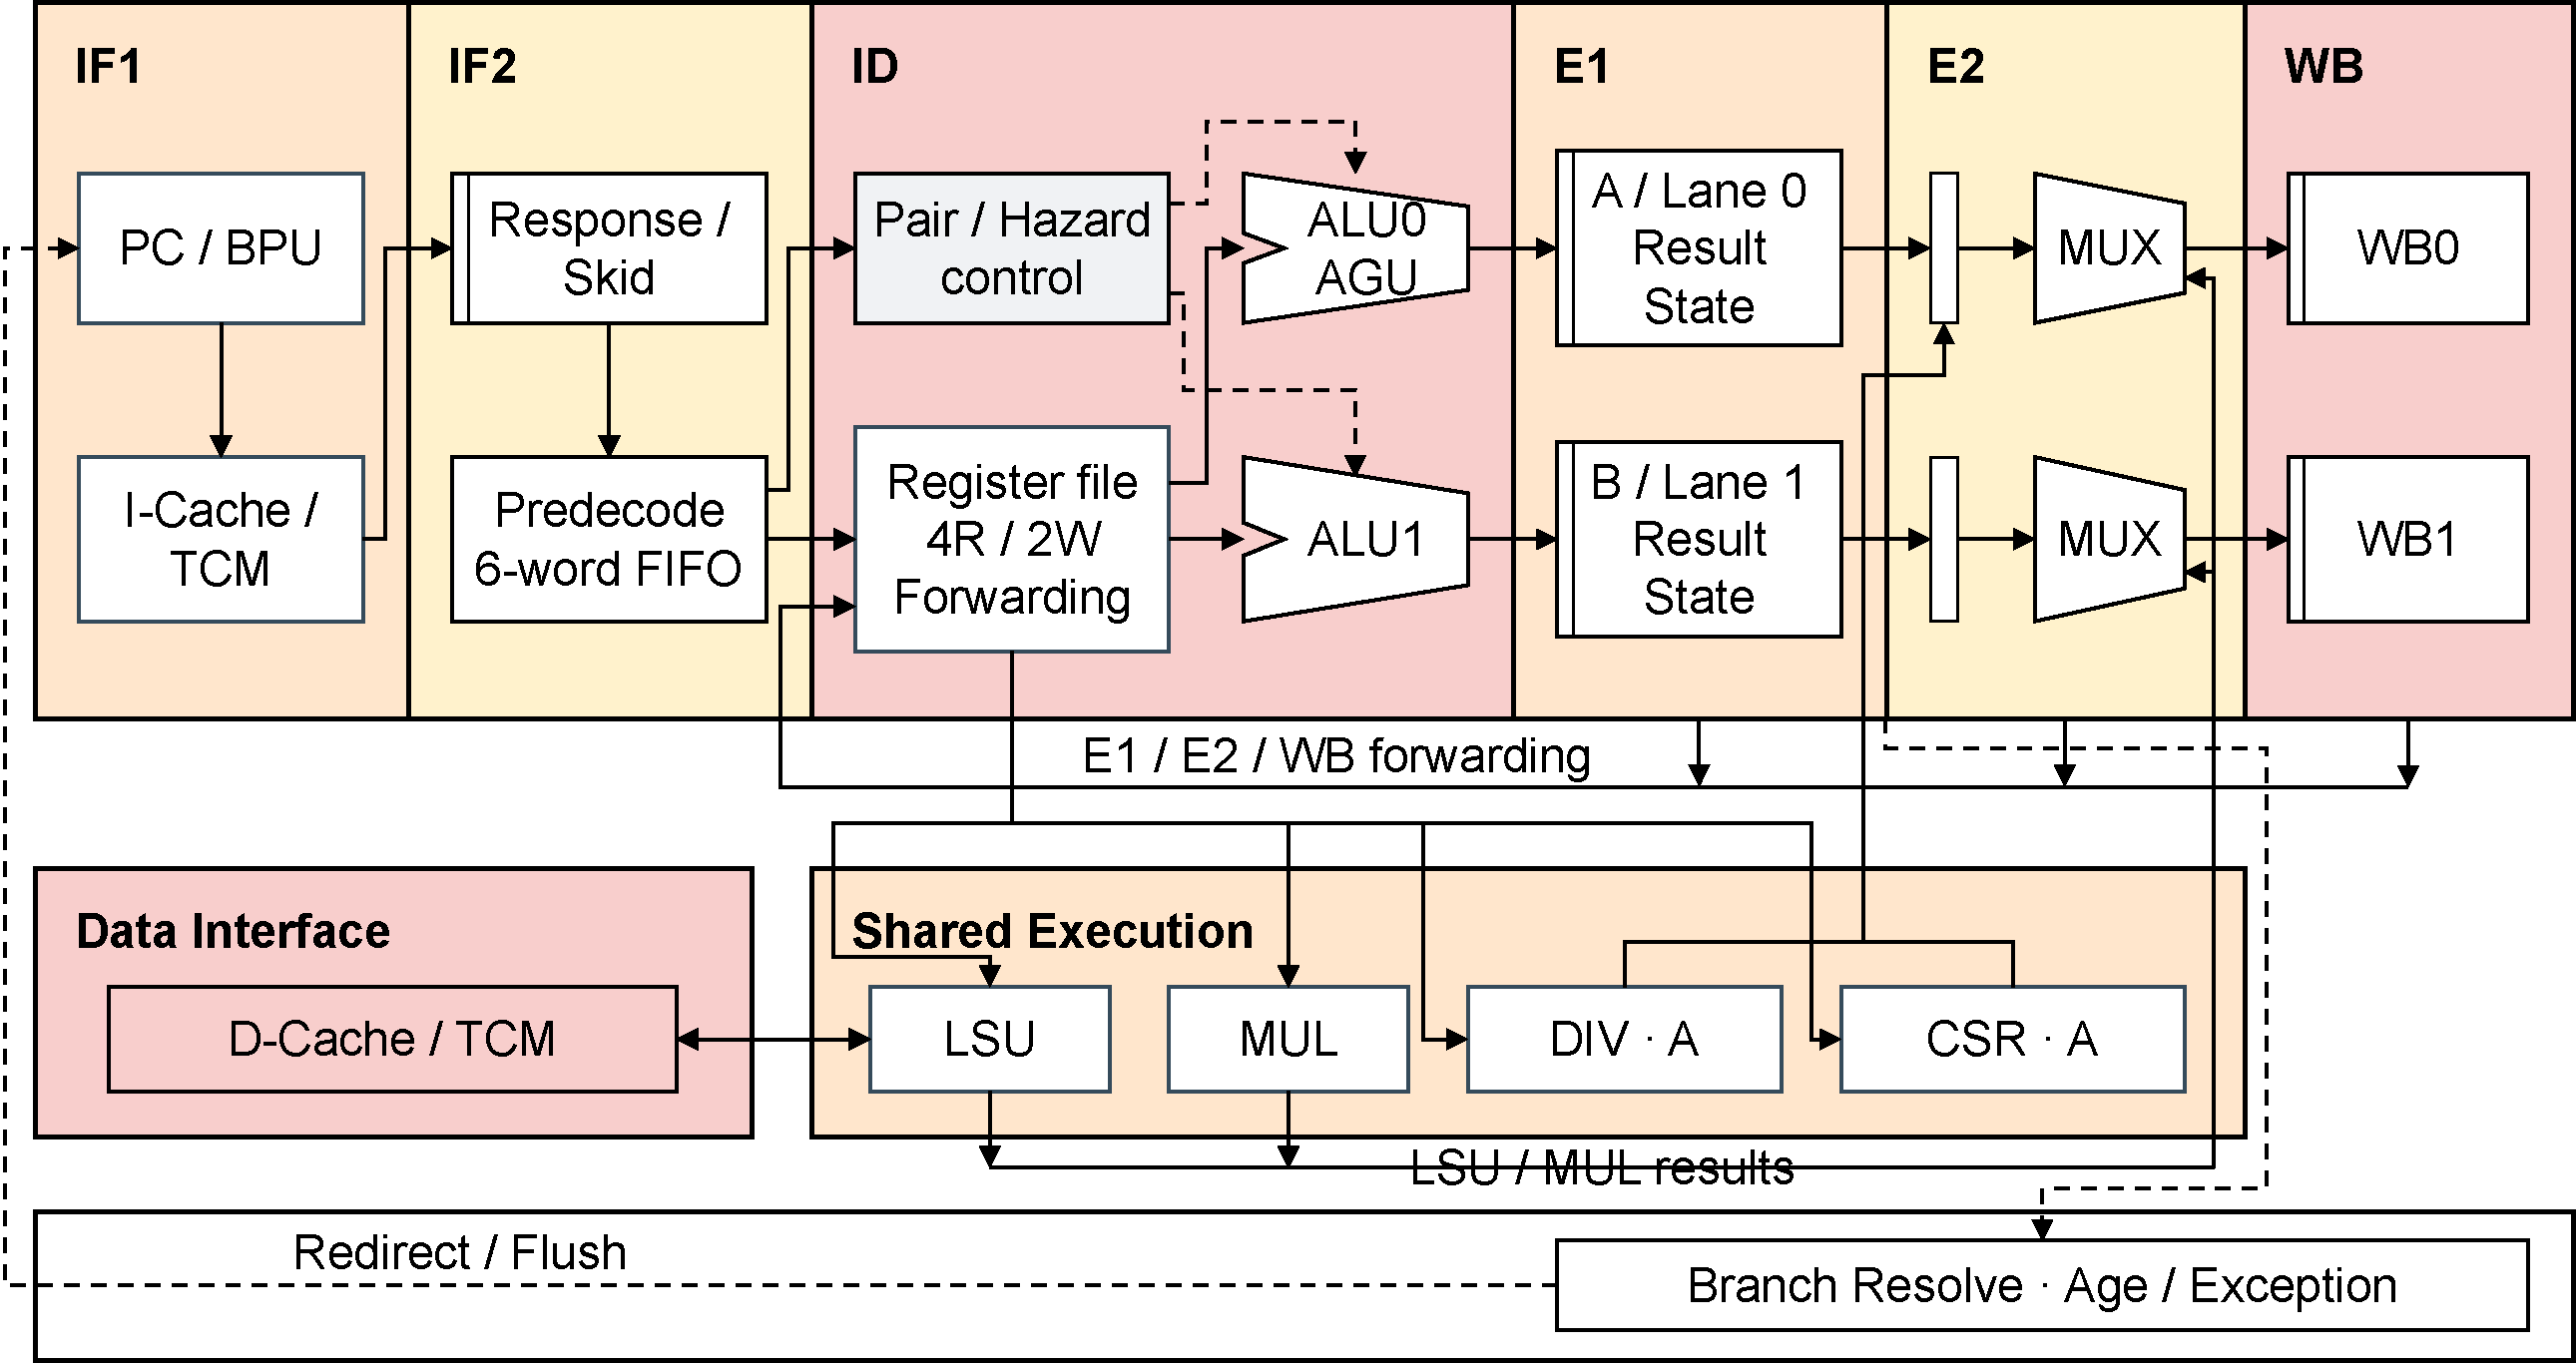
\includegraphics[width=\linewidth]{../figure/rv32-soc-page5.pdf}
\caption{六级CPU微架构}\label{fig:cpu-pipeline}
\end{figure}

\begin{reporttable}
\begin{longtable}{@{}p{0.18\linewidth}p{0.77\linewidth}@{}}
\caption{CPU实际流水级及寄存内容}\label{tbl:cpu-pipeline}\\
\toprule
流水级 & 功能与边界 \\
\midrule
\endfirsthead
\caption[]{CPU实际流水级及寄存内容（续）}\\
\toprule
流水级 & 功能与边界 \\
\midrule
\endhead
\bottomrule
\endfoot
IF1 & 选择顺序、预测或重定向地址，提交取指请求；接纳时保存PC及预测上下文 \\
IF2 & 接收返回包，匹配上下文，经响应缓冲和预译码写入指令FIFO \\
ID & 读取双队首，执行4路寄存器读取、前递及配对检查；计算ALU结果、访存地址和特定零比较分支的早期条件 \\
ID/E1边界 & 保存两条通路的指令状态、ALU结果、分支操作数、访存请求信息及乘法输入 \\
E1 & 解析通用分支，发出访存请求，提供整数结果前递及满足条件的低位乘积前递 \\
E2 & 获得常规乘法结果，接收访存完成或等待响应，选择各通路后续写回值 \\
WB & 根据有效位、异常及目的寄存器使能完成最多两路写回，并提供指令完成观测 \\
\end{longtable}
\end{reporttable}

各级状态包含PC、指令类型、有效位、目的寄存器及异常信息。暂停保持相关状态，恢复或异常控制撤销后续指令的有效性。
Cache未命中、总线背压及迭代除法会增加停留周期；双发射表示结构上限，实际吞吐率还受前端供给、数据相关和指令配对限制。
表\ref{tbl:cpu-pipeline}区分组合运算与寄存位置，避免将ALU结果寄存边界与分支解析阶段混为一谈。

\subsection{指令提取}

取指前端由PC选择、请求控制、预测器、请求上下文寄存器、响应缓冲和指令FIFO组成，如图\ref{fig:cpu-frontend}所示。
请求地址按8\,B对齐；每个64\,bit返回包包含两个32\,bit指令位置。入口PC的第2位保留在请求上下文中，用于确定第一条有效指令。

\begin{figure}[!htbp]
\centering
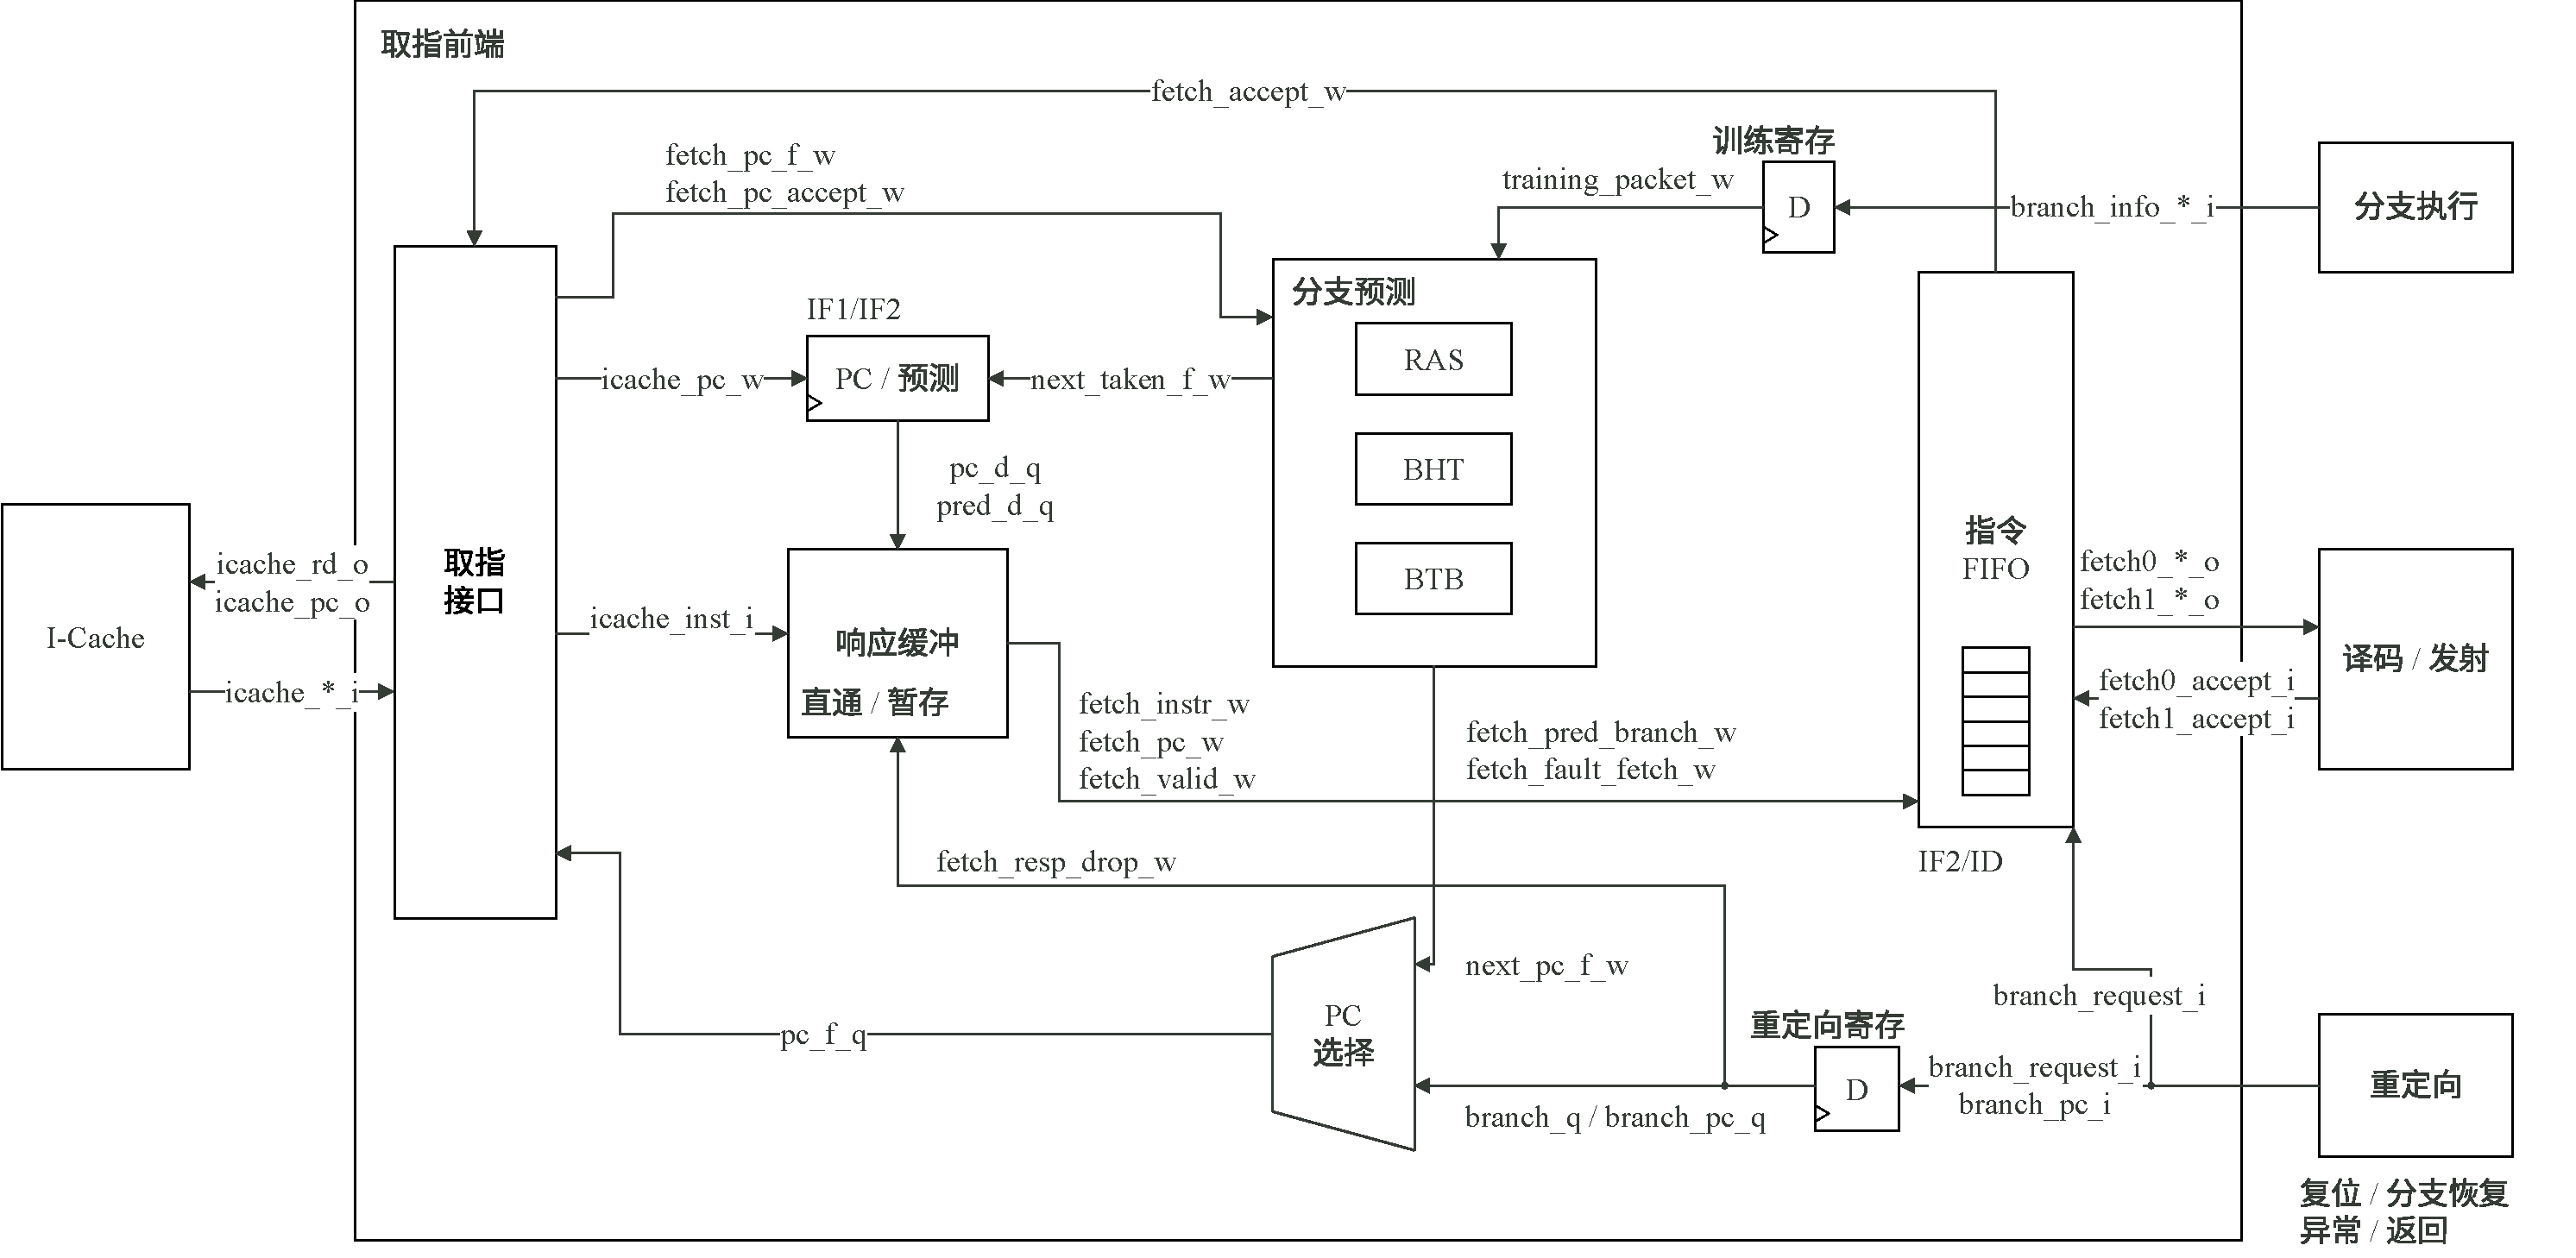
\includegraphics[width=\linewidth]{../figure/rv32-soc-page6.pdf}
\caption{取指前端的请求、返回与恢复通路}\label{fig:cpu-frontend}
\end{figure}

取指器跟踪一笔未返回请求。忙条件为“已有请求且本周期尚无有效响应”，因此前一响应到达时，可以在下层接纳和FIFO就绪均满足的情况下提交下一请求。
表\ref{tbl:fetch-overlap}给出一周期返回、无背压时的接口时序；它说明接口允许同周期接续，不表示所有缓存状态均能达到每周期一个包。
缓存查询延迟、未命中、重定向以及FIFO背压仍会降低实际供给率。

\begin{reporttable}
\begin{longtable}{@{}p{0.14\linewidth}p{0.35\linewidth}p{0.44\linewidth}@{}}
\caption{取指接口允许的理想接续时序}\label{tbl:fetch-overlap}\\
\toprule
周期 & 本周期接纳请求 & 本周期响应与上下文 \\
\midrule
\endfirsthead
\caption[]{取指接口允许的理想接续时序（续）}\\
\toprule
周期 & 本周期接纳请求 & 本周期响应与上下文 \\
\midrule
\endhead
\bottomrule
\endfoot
$T_0$ & 包0 & 无；沿后保存包0上下文 \\
$T_1$ & 包1 & 包0，使用沿前的包0上下文 \\
$T_2$ & 包2 & 包1，使用沿前的包1上下文 \\
$T_3$ & 包3 & 包2，使用沿前的包2上下文 \\
\end{longtable}
\end{reporttable}

132\,bit响应缓冲保存返回指令、PC、预测及错误状态。后端可接纳时直接传递，背压时保存完整返回包，解除背压后再送入FIFO。
已被接纳的旧取指请求不能由冲刷撤销总线事务，前端必须接收并丢弃其返回。
后端原始重定向在时钟沿清空FIFO，已寄存的重定向与延后一拍状态共同形成响应丢弃窗口；缓冲中的旧包同步失效。
表\ref{tbl:fetch-recovery}列出有旧请求在途时的事件关系，具体恢复请求周期由旧响应与下层接纳共同决定。

\begin{reporttable}
\begin{longtable}{@{}p{0.25\linewidth}p{0.34\linewidth}p{0.34\linewidth}@{}}
\caption{重定向与旧响应处理}\label{tbl:fetch-recovery}\\
\toprule
事件 & 前端动作 & 对后端可见的指令 \\
\midrule
\endfirsthead
\caption[]{重定向与旧响应处理（续）}\\
\toprule
事件 & 前端动作 & 对后端可见的指令 \\
\midrule
\endhead
\bottomrule
\endfoot
旧请求已接纳 & 保持旧PC及请求上下文 & 已在FIFO中的有效候选 \\
收到原始重定向 & 清空FIFO，寄存目标PC & 本沿取消旧队列状态 \\
恢复窗口内旧响应返回 & 丢弃旧响应，清除旧缓冲有效位 & 不向FIFO传递错误路径返回包 \\
恢复地址请求可接纳 & 提交目标PC，保存新上下文 & 等待新包返回 \\
目标包有效返回 & 经预译码重新入队 & 仅提供恢复路径候选 \\
\end{longtable}
\end{reporttable}

\subsubsection{分支预测}

分支预测器由分组BTB、两位计数器BHT、RAS及下一PC选择逻辑组成，如图\ref{fig:cpu-branch-prediction}所示。
BTB共512项，低字、高字各使用256项存储体，PC第10至3位索引行，第2位区分包内位置，高位地址用于标签匹配。
从低字入口查询时，低字命中优先，只有低字未命中才采用高字命中；从高字入口查询时仅采用高字结果。

\begin{figure}[!htbp]
\centering
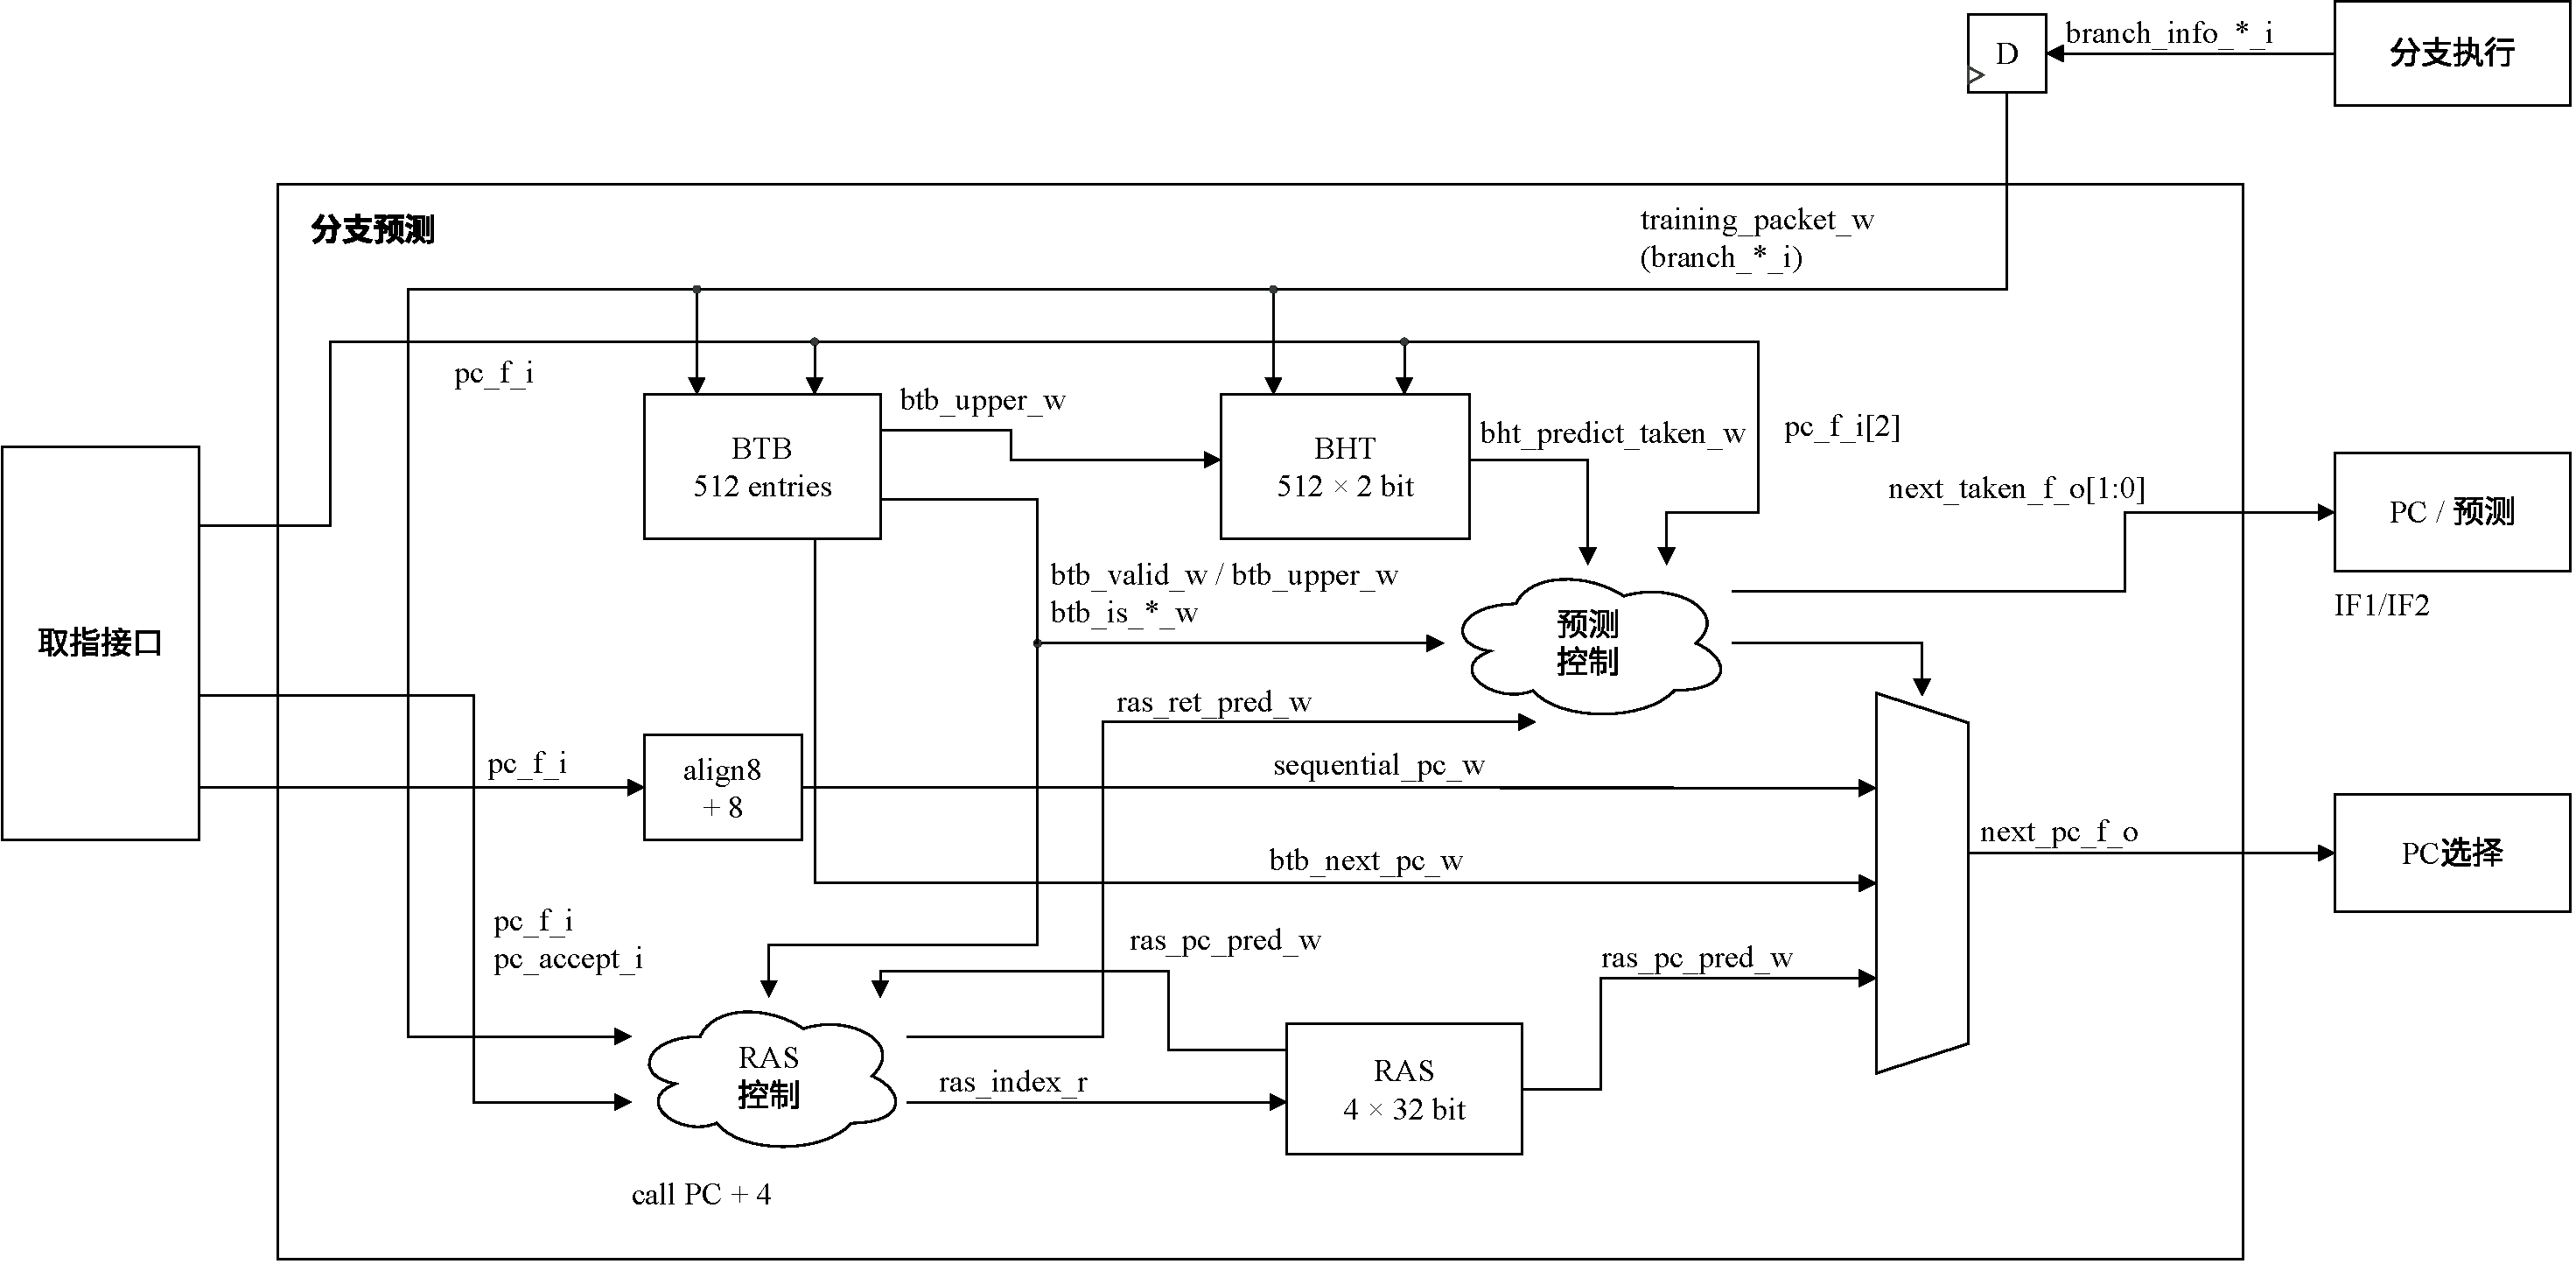
\includegraphics[width=\linewidth]{../figure/rv32-soc-page9.pdf}
\caption{分支目标、方向与返回地址预测结构}\label{fig:cpu-branch-prediction}
\end{figure}

BHT含512个两位饱和计数器，按BTB选中的指令位置选择方向预测，计数值2或3表示跳转。
训练按实际分支PC索引，跳转递增、不跳转递减，端点饱和。
这是一种先选择BTB命中位置、再判定该位置方向的结构：低字命中但预测不跳转时，不再重新选择高字的预测跳转。
因此该策略可能错过同包高字的提前跳转机会，后端仍按实际分支结果恢复PC。

RAS含4个32\,bit返回地址，以\texttt{x1}识别调用与返回，调用地址为该指令的$PC+4$。
预测调用或返回在PC通路可推进时更新推测栈指针；另一个参考指针在调用、返回的分支请求事件中参与修正。
执行通路解析真实分支目标，恢复控制在预测错误时纠正程序流。

有效返回预测优先使用RAS地址，其余跳转预测使用BTB目标；无跳转预测时采用$\operatorname{align8}(PC)+8$。
包内跳转标志区分低字、高字和无跳转，随请求上下文保存。低字预测跳转时，入队端不保留同包高字。
执行端的实际方向、目标、PC及类型通过分支事件寄存器训练预测器，BHT覆盖预测正确和错误的方向事件，BTB在恢复时分配或修正条目。

\subsubsection{指令FIFO}

图\ref{fig:fetch-fifo}中的FIFO按指令字组织，而非按取指包组织。六项环形存储提供六条指令容量，两个队首寄存器缓存最早的两个候选，二者不增加逻辑容量。
每项119\,bit载荷包含指令及取指状态、PC、预测下一PC、预译码信息和CSR提示。
取指入口位于包高字时，入队逻辑直接将高字作为第一条有效指令；不需要在发射端先丢弃一个低字。

\begin{figure}[!htbp]
\centering
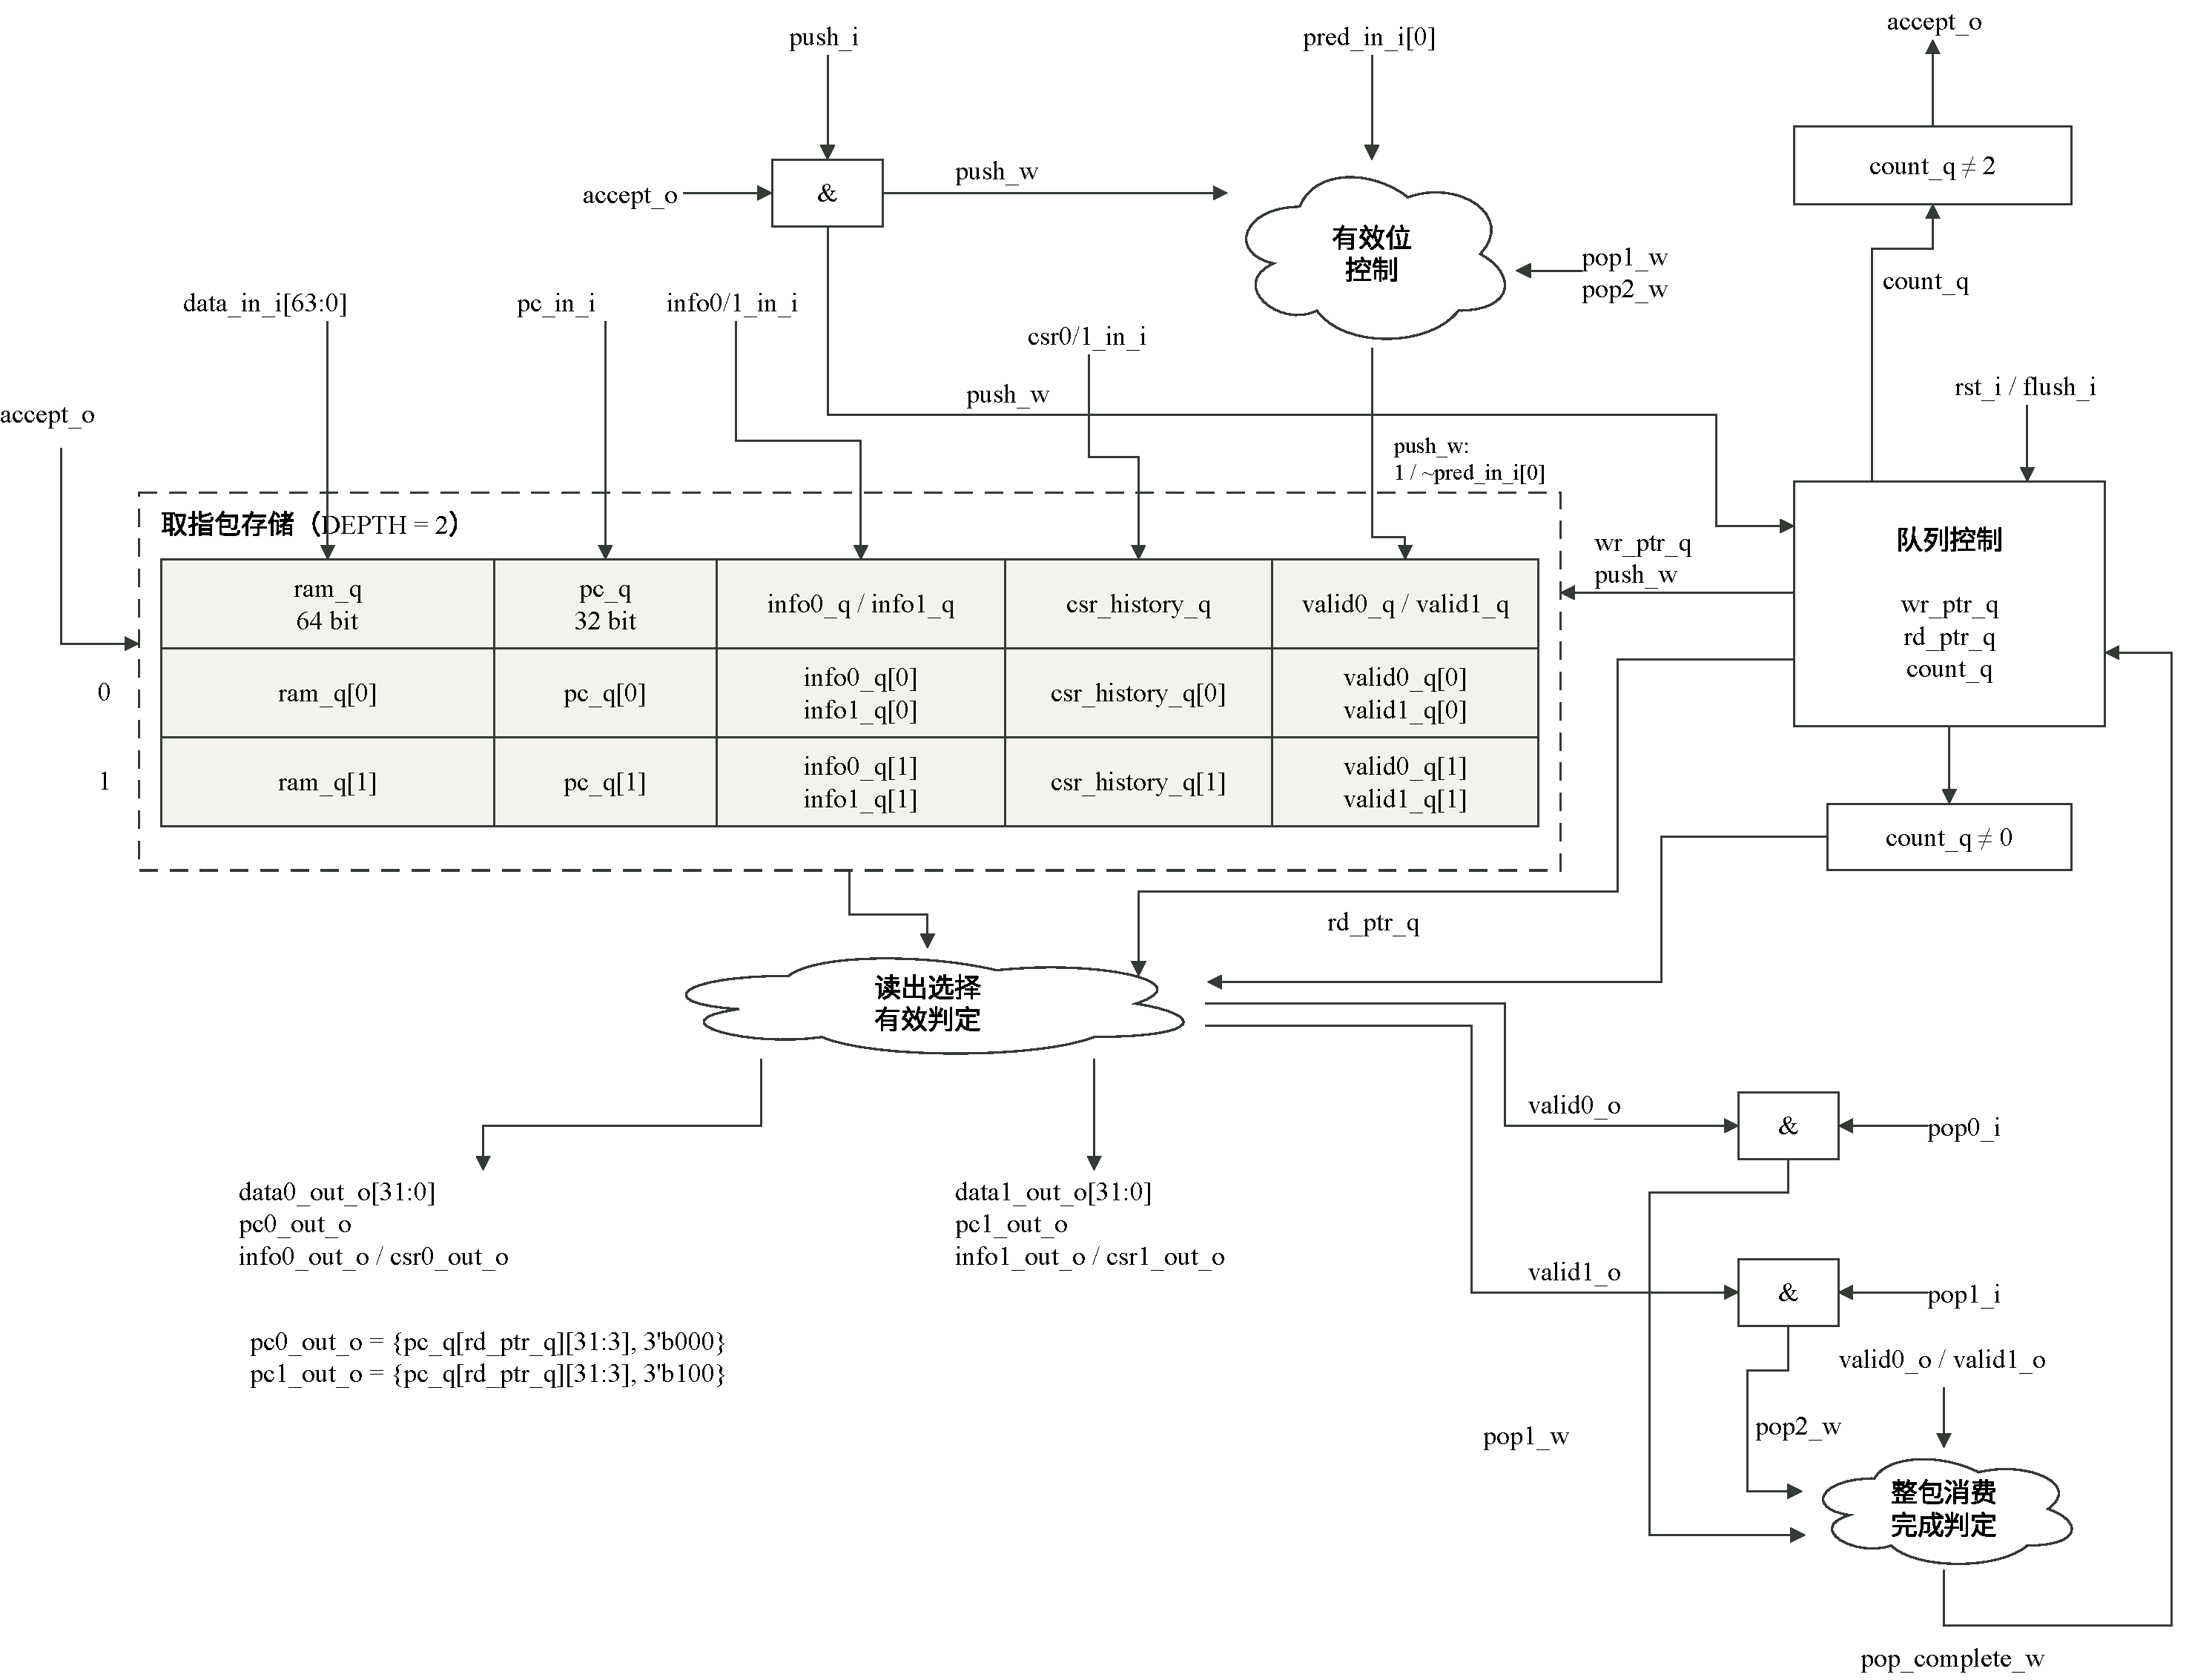
\includegraphics[width=\linewidth]{../figure/rv32-soc-page10.pdf}
\caption{六项指令FIFO与双队首顺序出队}\label{fig:fetch-fifo}
\end{figure}

入队根据入口位置和包内预测标志写入一条或两条指令。就绪条件为当前占用数不超过4，预留最多两条输入的容量；本周期出队释放的容量不提前计入接纳余量。
Head0始终对应程序顺序最靠前的候选A，Head1对应后继候选B；只有两者PC相差4且其他配对条件成立，才允许共同发射。
因此队首可以跨越取指包边界，示例见表\ref{tbl:fifo-cross-packet}。

\begin{reporttable}
\begin{longtable}{@{}p{0.23\linewidth}p{0.28\linewidth}p{0.42\linewidth}@{}}
\caption{跨取指包配对示例}\label{tbl:fifo-cross-packet}\\
\toprule
事件 & 队首A、B & 更新结果 \\
\midrule
\endfirsthead
\caption[]{跨取指包配对示例（续）}\\
\toprule
事件 & 队首A、B & 更新结果 \\
\midrule
\endhead
\bottomrule
\endfoot
包$P$与$P+8$已入队 & $P$、$P+4$ & 环中后续为$P+8$、$P+12$ \\
仅A可发射 & $P$出队，B保留 & 新队首为$P+4$、$P+8$ \\
新队首可配对 & $P+4$、$P+8$ & 同周期出队，虽来自不同取指包仍保持程序顺序 \\
发生恢复冲刷 & 所有候选失效 & 计数和队首状态复位；载荷RAM无需逐项清零 \\
\end{longtable}
\end{reporttable}

CPU的出队约束为$\mathrm{pop1}\Rightarrow\mathrm{pop0}$：B出队必须伴随A出队。
队首更新分别选择保留或前移的Head0/Head1、环形存储中rd+2/rd+3处的后续项，以及本周期输入旁路。
两路Next选择器形成下一周期队首载荷；队首数据、占用数及指针共同决定候选有效性。
更新时冲刷优先于入队、出队；正常周期按实际入队数和出队数更新占用及队首。
恢复沿可能同时存在队列出队条件的组合计算，但最终执行请求已被恢复控制屏蔽，队列状态以冲刷为准。

\subsection{指令译码}

译码与发射结构如图\ref{fig:cpu-decode-issue}所示，为A、B通路提供指令与就绪操作数。两条候选各提供两个寄存器索引，逻辑4读2写寄存器堆与E1/E2/WB前递网络并行提供操作数。
寄存器\texttt{x0}读零且不建立写入依赖。同一源寄存器对应多个前序写入指令时，按程序顺序选择最近的写入结果；该结果尚未就绪时阻止发射。
同一对中的A写B读相关以及A/B同目的寄存器冲突都会禁止B发射，保留B为后续周期的队首。

\begin{figure}[!htbp]
\centering
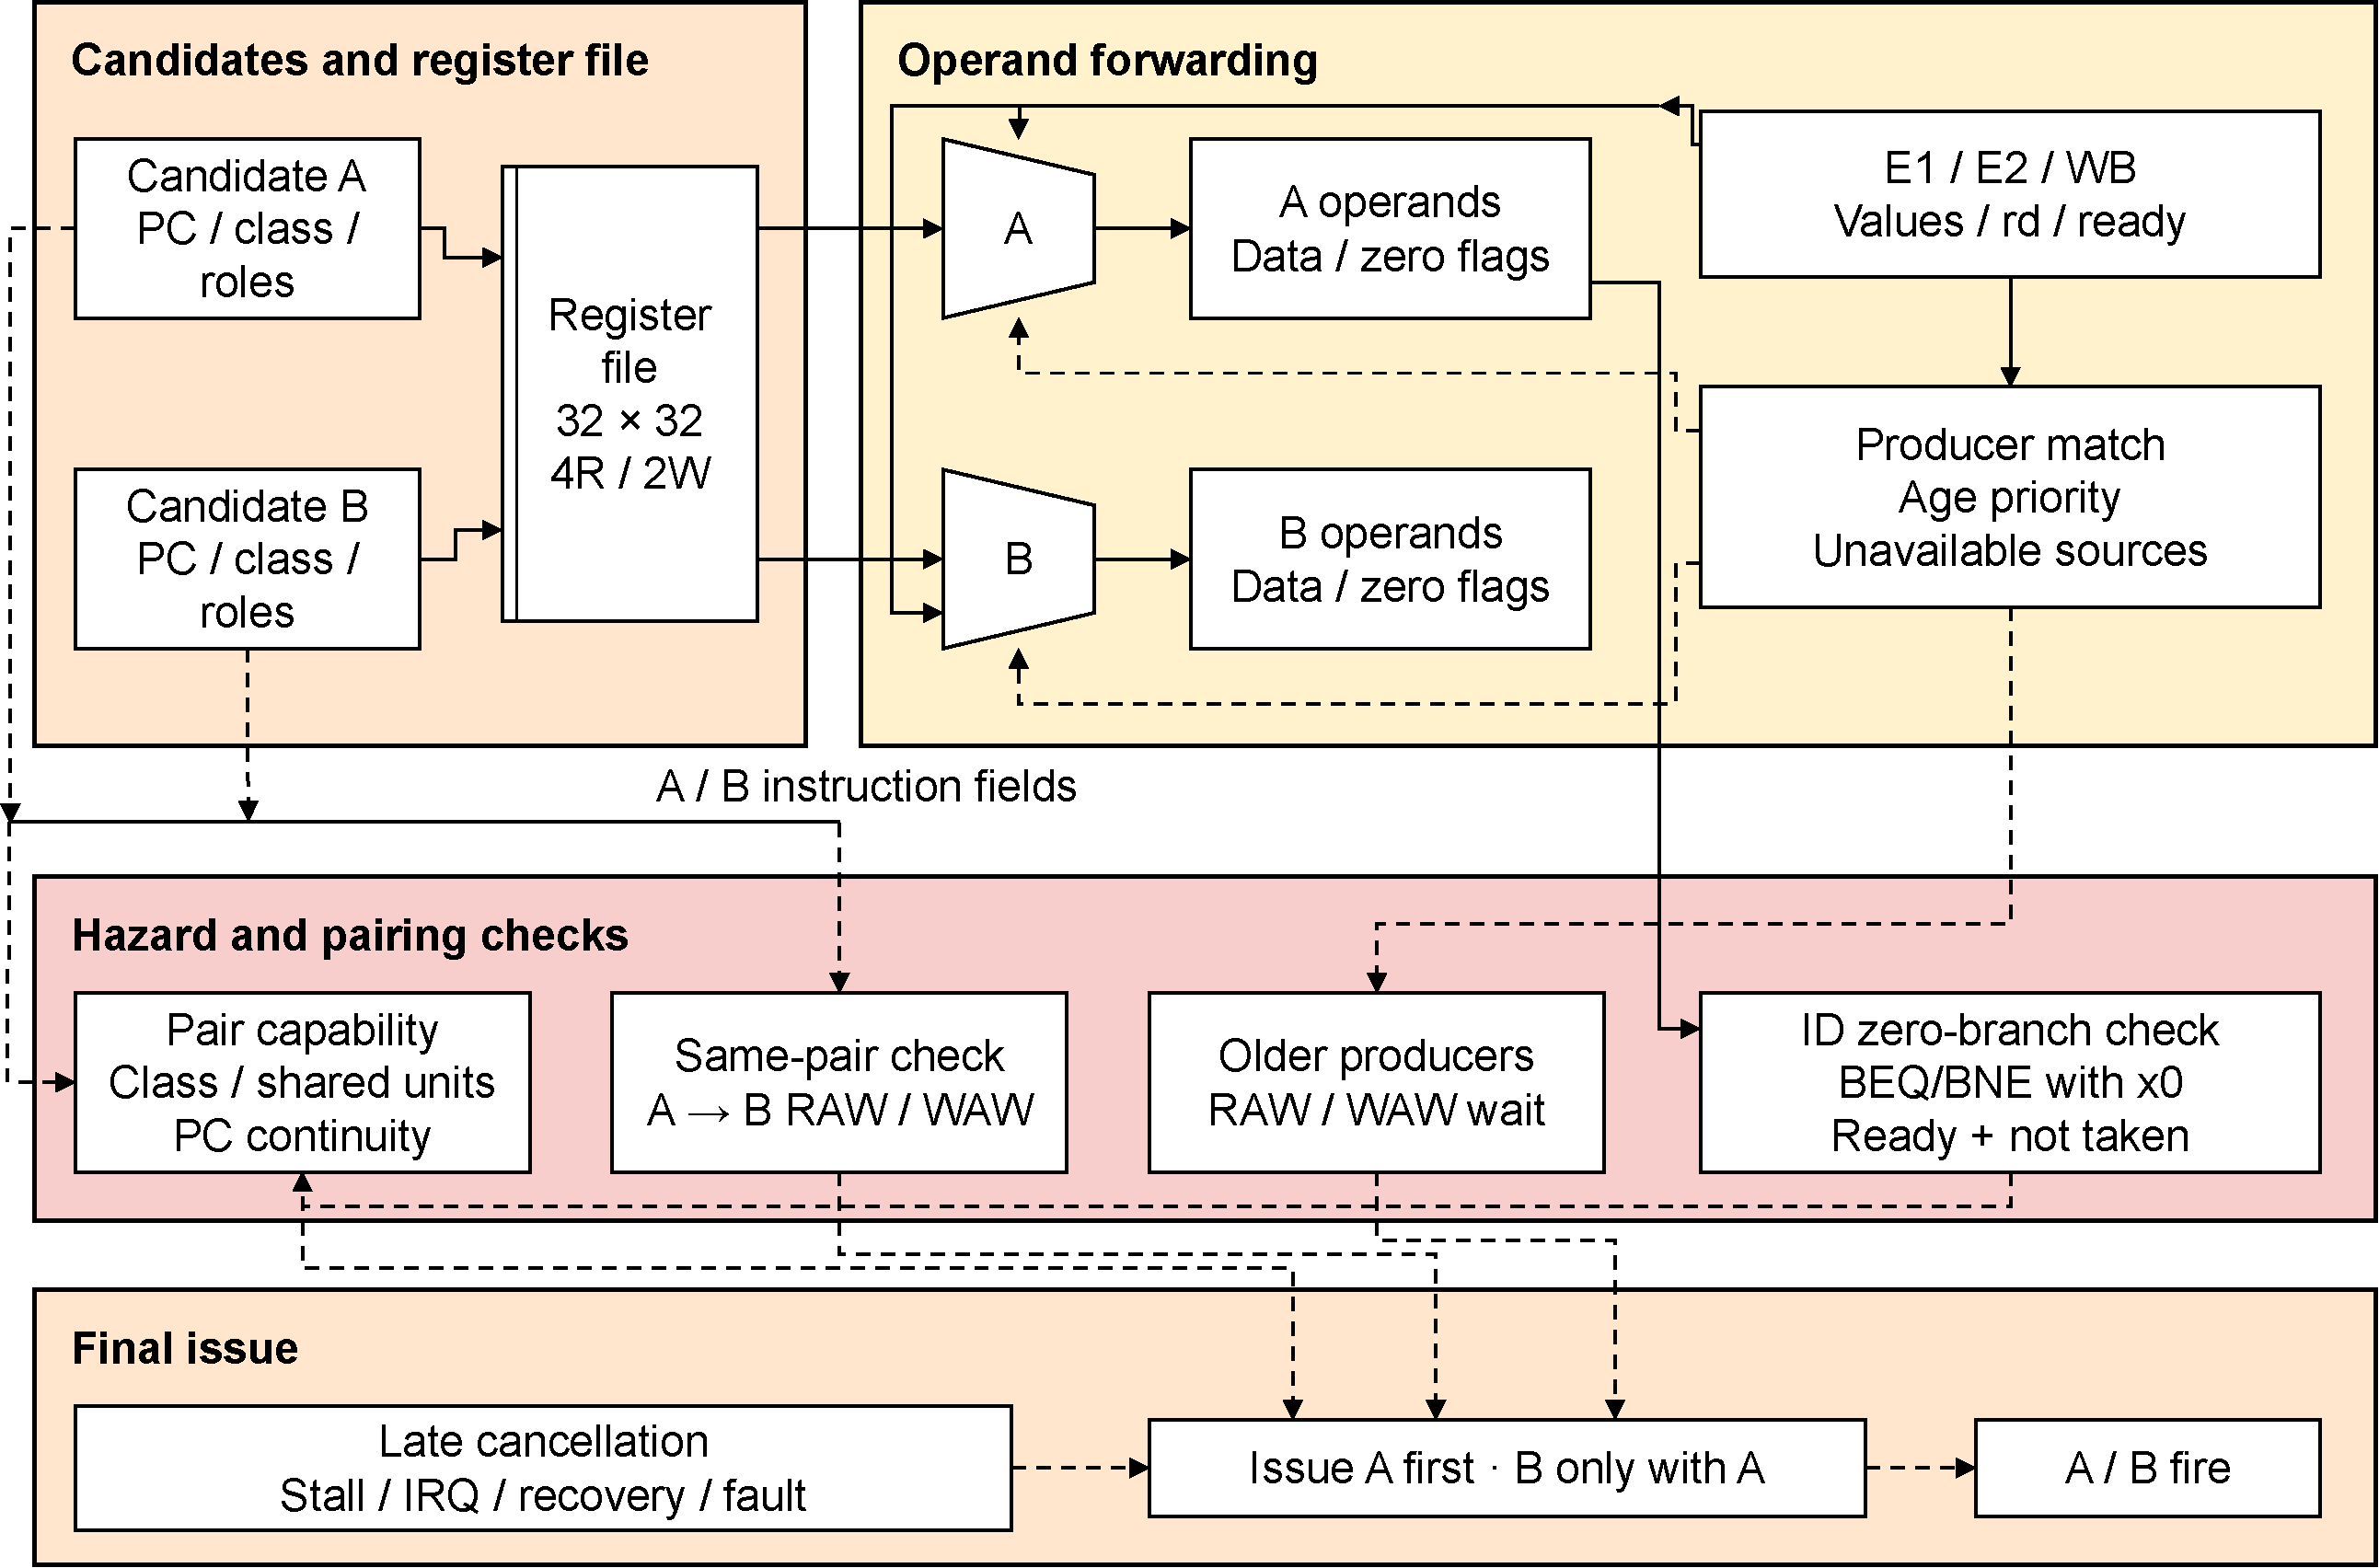
\includegraphics[width=\linewidth]{../figure/rv32-soc-page11.pdf}
\caption{双候选译码、操作数前递与发射控制}\label{fig:cpu-decode-issue}
\end{figure}

\subsection{指令执行}

双执行通路与共享资源如图\ref{fig:cpu-execute}所示。两路ALU的组合结果分别在ID/E1边界锁存。各通路的E2寄存状态继续保存结果、类型与有效信息；A槽在进入E2时选择ALU、DIV或CSR结果，随后由E2结果选择逻辑接入LSU或MUL返回，并送入WB。EX0支持完整整数运算，EX1支持加减、逻辑、比较和立即数移位，不接收寄存器变量移位。

\begin{figure}[!htbp]
\centering
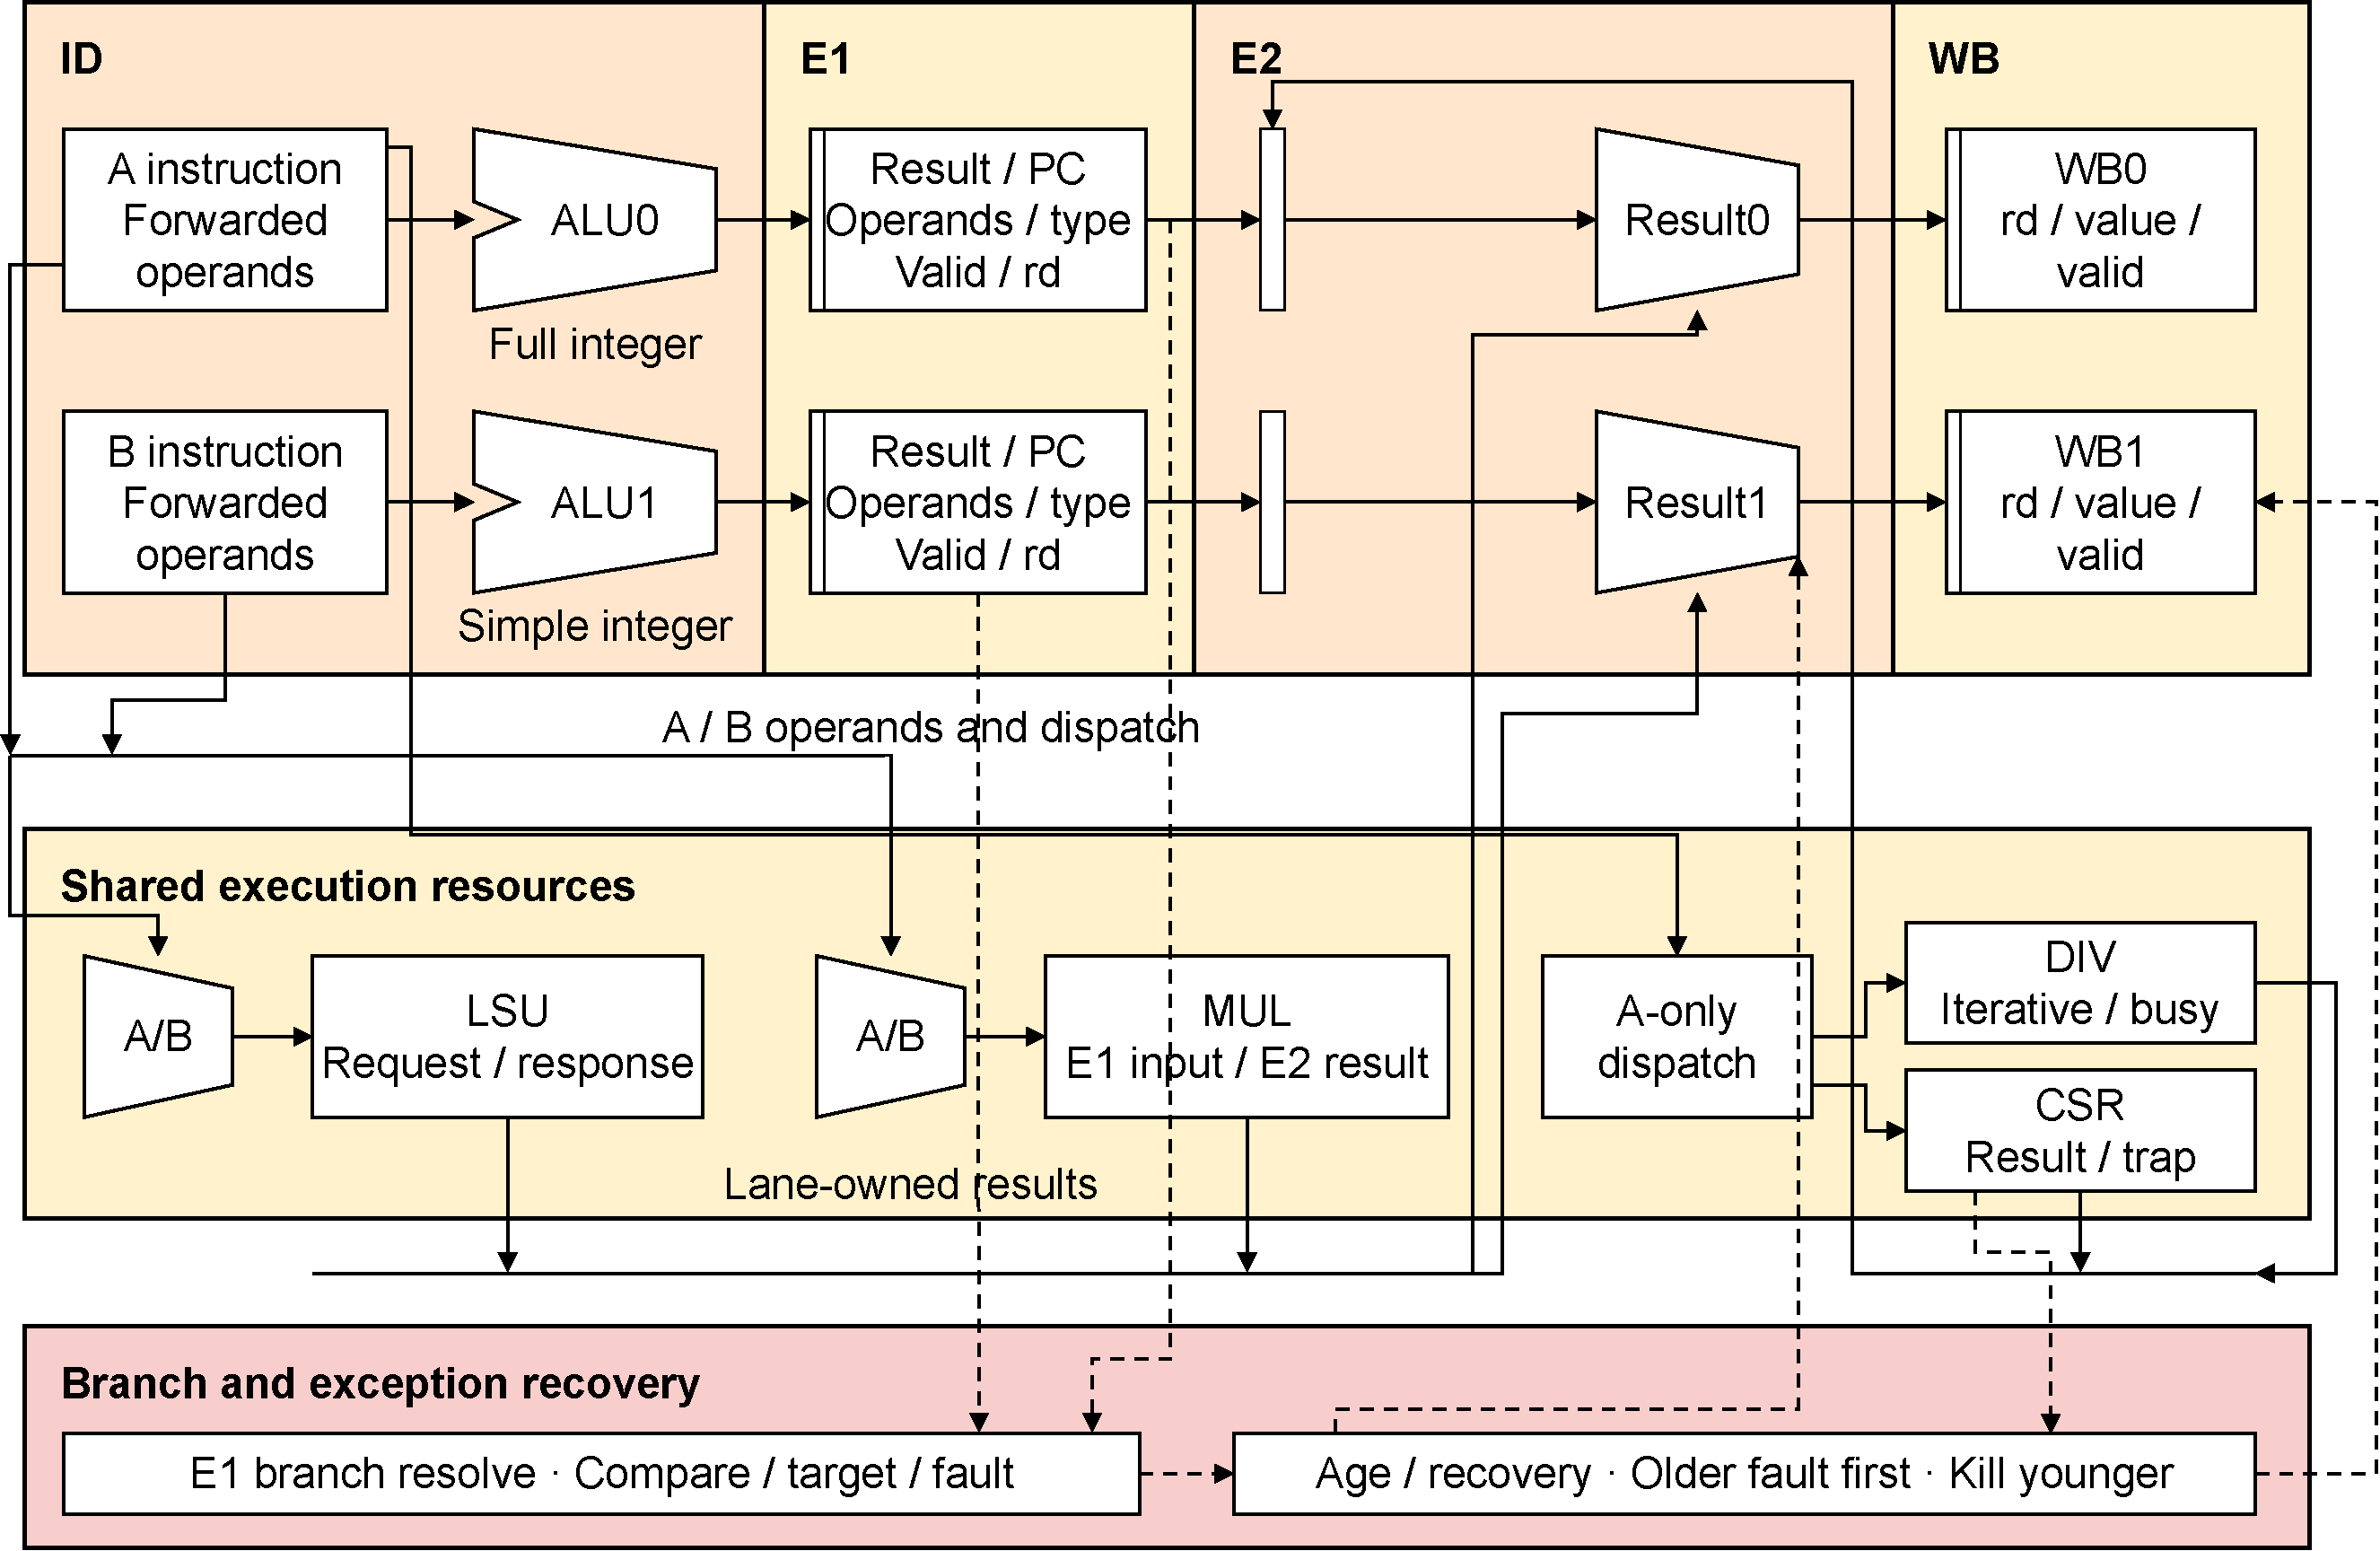
\includegraphics[width=\linewidth]{../figure/rv32-soc-page12.pdf}
\caption{双执行通路、共享资源与恢复控制}\label{fig:cpu-execute}
\end{figure}

整数ALU的数据通路如图\ref{fig:cpu-alu}所示。输入根据指令选择寄存器值、PC或立即数，
加减、比较、逻辑及移位结果经选择后在ID/E1边界写入结果寄存器，两条执行通路分别使用独立实例。
暂停时保持结果寄存器，指令有效性由流水控制管理，寄存器中的数据本身不表示有效指令。

\begin{figure}[!htbp]
\centering
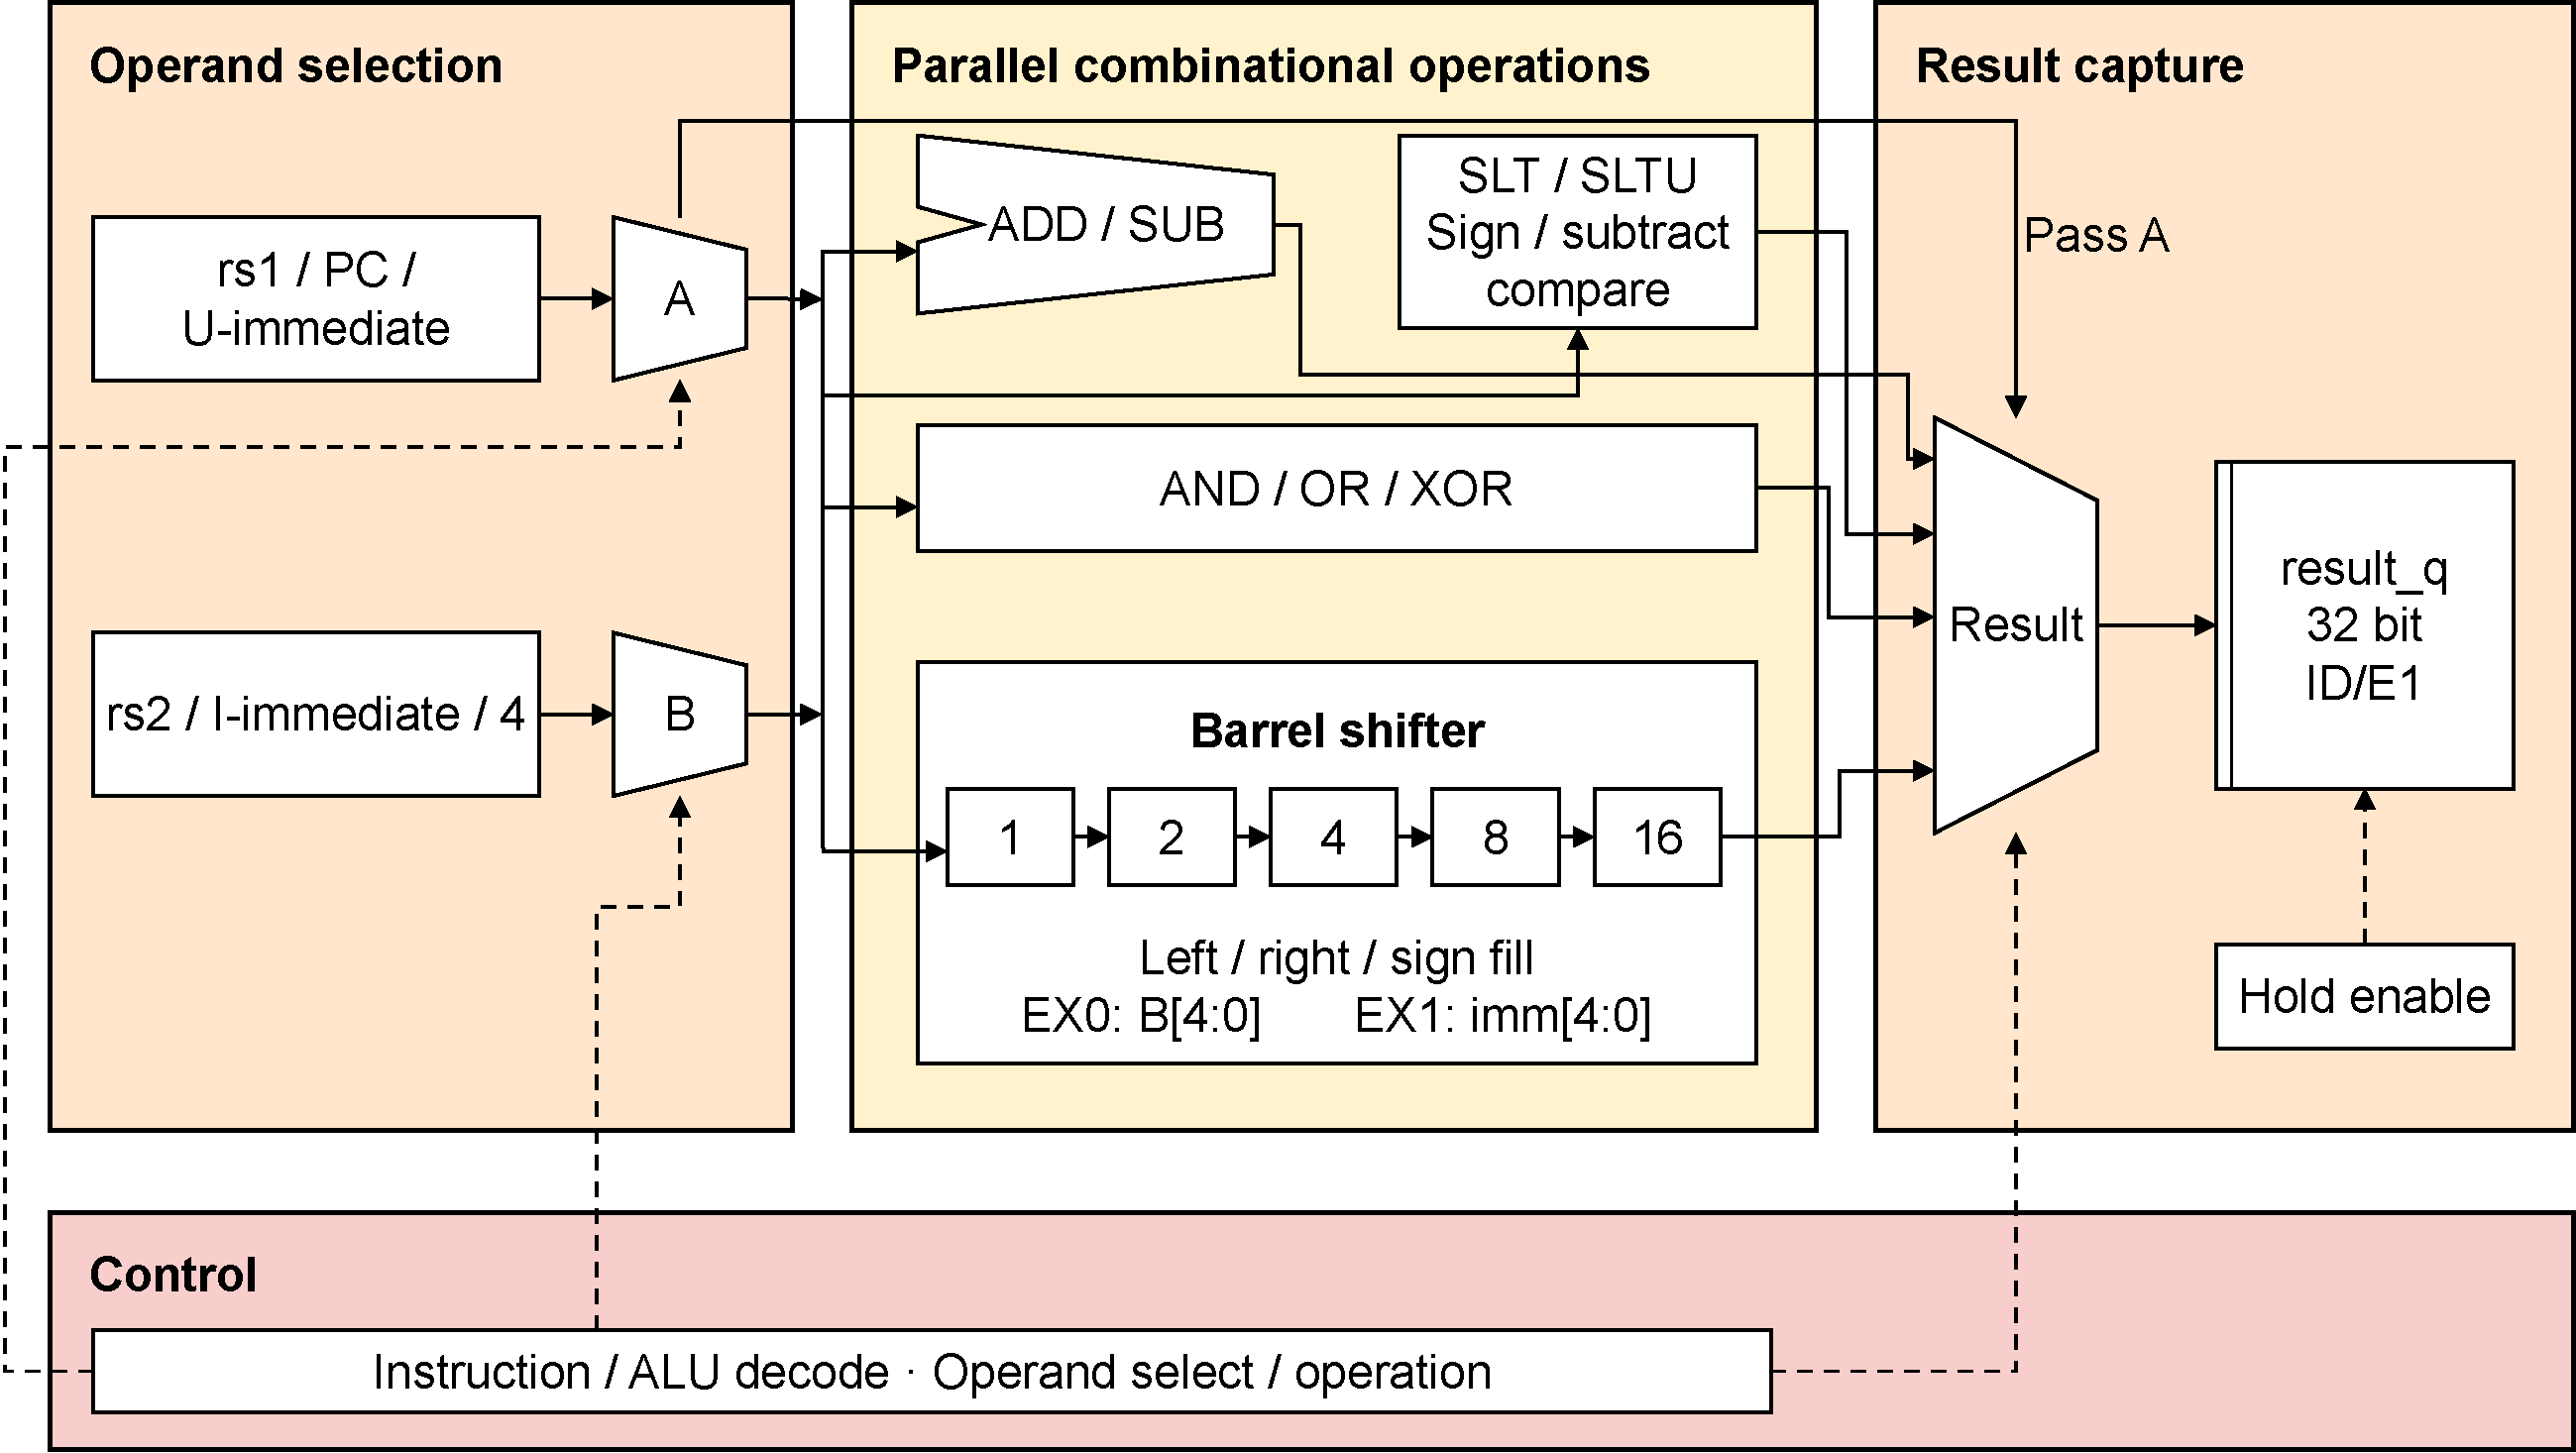
\includegraphics[width=\linewidth]{../figure/rv32-soc-page13.pdf}
\caption{整数ALU组合通路及ID/E1结果寄存边界}\label{fig:cpu-alu}
\end{figure}

LSU与MUL各自独立选择A或B的指令和操作数，因此LSU与MUL可在同周期分别接收一条指令；单个共享单元不能同时接收A与B。
DIV和CSR只使用A槽，执行期间通过在途状态串行化相关控制。表\ref{tbl:issue-pairing}给出资源层面的允许组合，所有组合还需满足PC连续、操作数就绪、无相关冲突且A槽指令被接纳。

\begin{reporttable}
\begin{longtable}{@{}p{0.27\linewidth}p{0.35\linewidth}p{0.31\linewidth}@{}}
\caption{双发射配对规则}\label{tbl:issue-pairing}\\
\toprule
A槽类型 & 允许的B槽类型 & 附加约束 \\
\midrule
\endfirsthead
\caption[]{双发射配对规则（续）}\\
\toprule
A槽类型 & 允许的B槽类型 & 附加约束 \\
\midrule
\endhead
\bottomrule
\endfoot
整数ALU & 简单ALU、分支、LSU、MUL & B须属于EX1或共享单元支持的类型 \\
LSU & 简单ALU、分支、MUL & 不允许第二条LSU \\
MUL & 简单ALU、分支、LSU & 不允许第二条MUL \\
未提前判定的分支 & 简单ALU & B仅作推测运算，A恢复或故障时取消B \\
ID确认不跳转的BEQ/BNE零比较 & 简单ALU、LSU、MUL & A、B有效且无取指或非法指令错误；零标志对应就绪的前递操作数 \\
DIV或CSR & 无 & 仅A槽发射 \\
\end{longtable}
\end{reporttable}

ID中的早期分支检查只处理BEQ/BNE且至少一个源寄存器为\texttt{x0}的情况。
另一操作数的零标志与数据使用相同的前递来源和优先级；BEQ比较值非零、BNE比较值为零时，可以在ID确认不跳转。
该判断只确定是否允许配对，最终发射仍检查尚未完成的前序写入指令、同对相关、全局暂停、异常及中断取消条件。
未就绪加载或乘法的暂态零标志不能单独授权B，普通双操作数分支也不使用此早期通路。

A分支尚未在ID确定不跳转时，B仅可为简单ALU。A在E1解析出恢复或故障时，\texttt{cancel1\_e1}取消B向E2推进，避免其写回。
允许B进入LSU的零比较分支组合由ID条件提前授权，不依赖同周期尚未产生的E1结果；LSU实际有效脉冲还由最终发射和中断屏蔽共同限定。
已经被存储接口接纳的Store没有通用撤销机制，因而禁止错误路径Store发出必须发生在接纳之前。

A为Load、B为分支时，共享暂停保持两条指令的状态及其对应执行通路，分支恢复不能越过尚未完成的A槽加载访问。
前序访存指令的异常取消后续指令，CSR异常或返回重定向优先于普通分支恢复。
通用条件分支的比较与目标生成使用E1寄存的操作数、PC和指令；跳转链接值为$PC+4$，目标按4\,B指令边界检查。
分支解析、队列冲刷和后续指令取消共同恢复程序流，不能仅依靠预测器保持正确执行。

乘法器支持\texttt{MUL/MULH/MULHSU/MULHU}，输入在E1保存，常规结果在E2保存。
启用相应早期旁路时，\texttt{MUL}且两个输入高16位均为零，可从E1输入形成组合低位部分积供后继相关指令使用；完整结果仍通过E2正常写回。
高位乘法和不满足范围条件的低位乘法继续等待常规结果，不使用早期值。
除法器按迭代方式生成商和余数，包含除零及有符号溢出的规定结果；完成前保持在途状态。
CSR采用专用读改写和异常控制通路，整数寄存器写回值与CSR副作用分别管理。

\subsection{存储访问}

LSU结构见图\ref{fig:cpu-lsu}。地址生成将基址与I型或S型立即数相加，访问控制译码字节宽度、符号扩展及缓存属性。
字节访问允许任意字节地址，半字与字访问分别要求低1位、低2位为零；不对齐时禁止外部读写，使用内部完成事件报告异常。
Store按有效地址低位排列数据并生成4\,bit字节使能。请求信息在ID/E1边界保存，由E1向D-Cache或TCM提交。

\begin{figure}[!htbp]
\centering
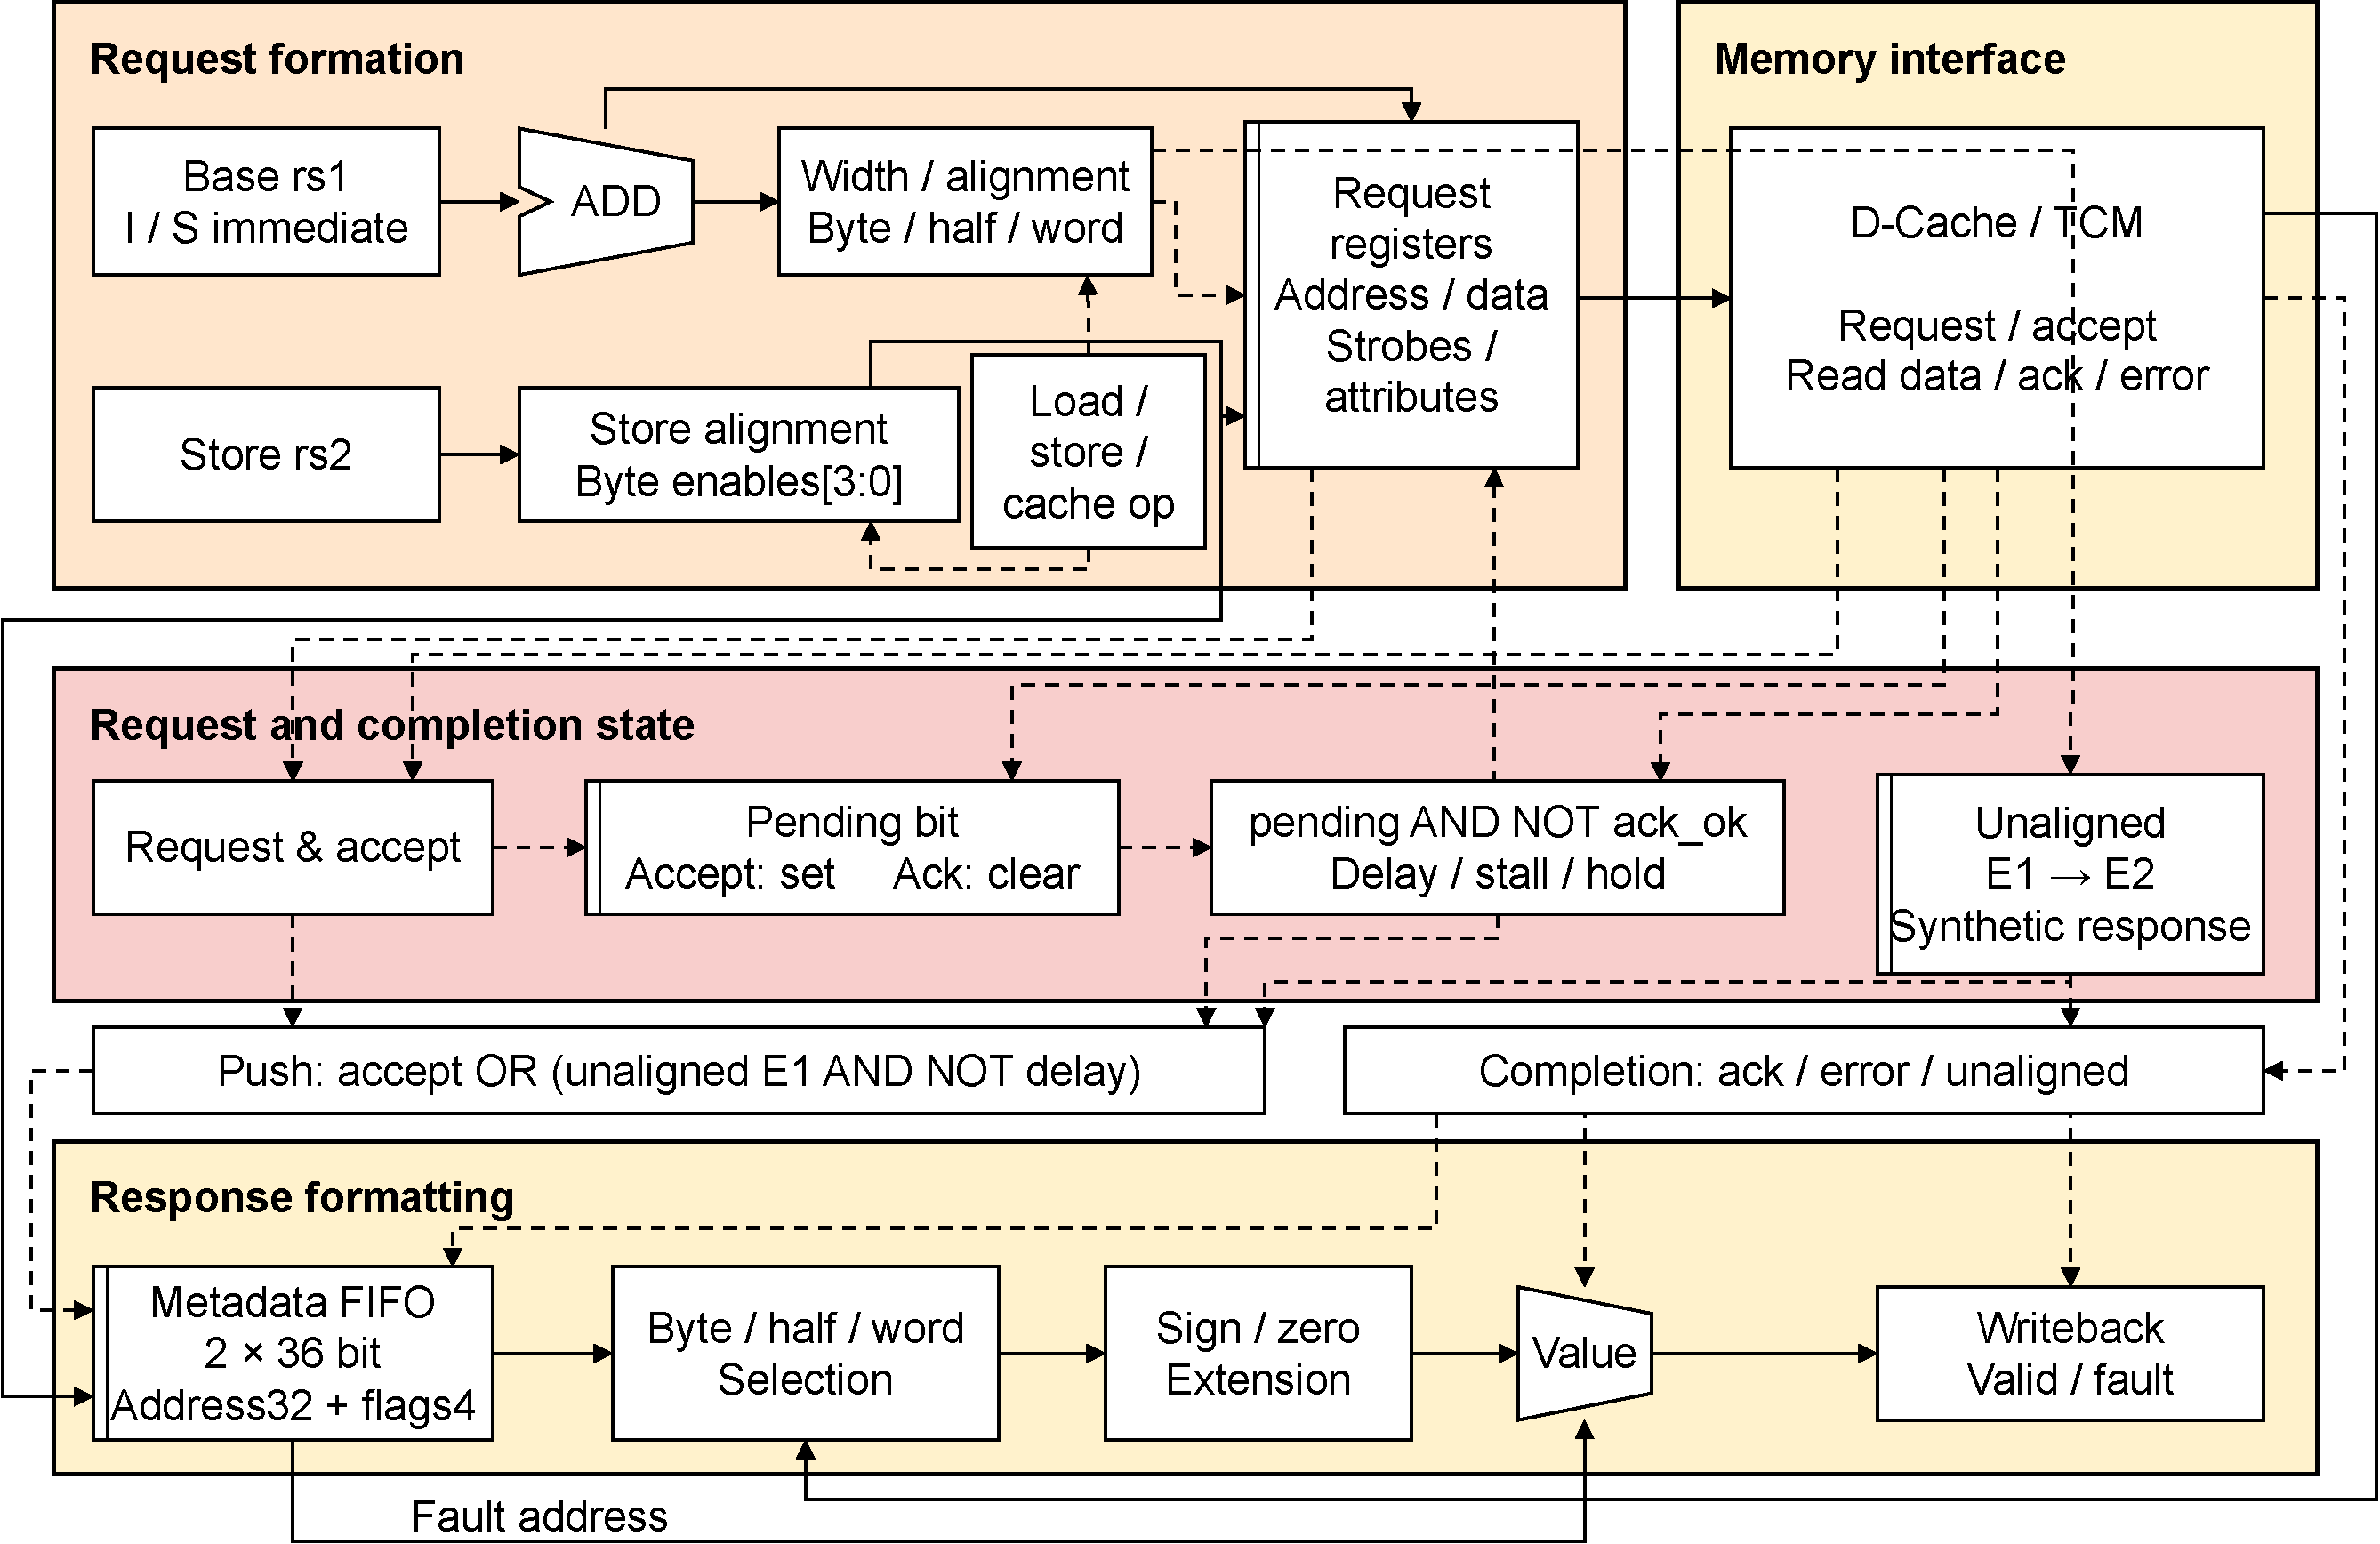
\includegraphics[width=\linewidth]{../figure/rv32-soc-page14.pdf}
\caption{LSU请求、数据处理与完成通路}\label{fig:cpu-lsu}
\end{figure}

请求接纳和访问完成是两个事件：\texttt{mem\_accept}接纳请求，\texttt{mem\_ack}报告响应，\texttt{mem\_error}报告访问错误。
未接纳期间保持请求；接纳后设置pending，等待完成时阻止继续接纳新的外部事务。成功完成与下一次接纳可在同一周期交接，见表\ref{tbl:lsu-handoff}。
表中状态取时钟沿前后，例子假定下一请求已准备且没有异常、背压或其他流水阻塞。

\begin{reporttable}
\begin{longtable}{@{}p{0.13\linewidth}p{0.20\linewidth}p{0.29\linewidth}p{0.31\linewidth}@{}}
\caption{LSU成功响应与下一请求接纳的交接}\label{tbl:lsu-handoff}\\
\toprule
周期 & 沿前状态 & 接口事件 & 沿后状态 \\
\midrule
\endfirsthead
\caption[]{LSU成功响应与下一请求接纳的交接（续）}\\
\toprule
周期 & 沿前状态 & 接口事件 & 沿后状态 \\
\midrule
\endhead
\bottomrule
\endfoot
$T_0$ & 无待完成访问 & 接纳请求A & pending=1，队首为A元数据 \\
$T_1$ & A等待响应 & 无ack，无新接纳 & 保持A对应的执行通路及流水状态 \\
$T_2$ & A等待响应 & ack(A)与accept(B) & A完成并出队，B入队；pending保持1 \\
$T_3$ & B等待响应 & 无ack，无新接纳 & 保持B对应的执行通路，不重复接纳B \\
$T_4$ & B等待响应 & ack(B)，无新接纳 & B出队，pending清零 \\
\end{longtable}
\end{reporttable}

请求元数据FIFO深度为2，每项保存32\,bit地址和加载、字节、半字、符号扩展四个标志，共36\,bit。
外部请求被接纳时元数据入队；非对齐E1事件在未被延迟时也入队，以便内部完成事件取得相应故障地址。
外部ack或非对齐E2事件弹出队首。
这一容量服务元数据保存与同周期出入队，不表示总线允许两笔独立未完成事务。
请求标签固定为零；元数据不包含发射槽、目的寄存器或PC，Pipe0/Pipe1通过其在途类型、有效位和共享暂停，保持返回结果与对应流水线的关联。
响应周期按旧队首格式化A数据，时钟沿再弹出A并写入B；pending更新中接纳优先于完成清除，保持新请求的等待状态。

加载返回选择目标字节、半字或整字并执行符号或零扩展，成功结果送入对应流水线，并在满足旁路条件时用于前递。
访问错误或内部非对齐完成携带故障地址及异常原因，取消正常目的寄存器更新。
请求寄存器接纳后撤销该次请求的有效状态，下一事务只有在新的有效发射和请求握手成立时才接纳。
已接纳事务继续完成接口协议，恢复控制负责抑制被取消指令的正常写回。

可缓存Store在D-Cache完成选中字节更新与脏位置位后得到响应，脏数据通过替换或维护写回DDR；不可缓存Store等待下层写事务完成。
共享DMA数据使用不可缓存区，根据成功写响应、访问顺序及所有权移交状态确定读取方何时可访问数据。

\subsection{指令写回}

双发射配置的两条通路分别保持E1、E2和WB的指令状态，在WB按有效位、异常与目的寄存器使能提供最多两路寄存器写入；单发射配置仅由A通路写回。
同对指令保持A先B后的程序顺序，前序指令异常和恢复控制取消不应提交的后续指令。
Store及分支等无通用寄存器写入的指令仍有完成事件，不能以寄存器写使能代替退休数量。
仿真在相同计时窗口采样两条通路的有效完成信息和周期数，IPC按该窗口内完成指令总数除以周期数计算。

\subsection{流水线控制}

前递网络从两条通路的E1、E2及WB中选择程序顺序最近的前序写入结果；E1整数结果可立即前递，Load及普通MUL需等待对应完成阶段。
记分牌与源角色信息过滤无效寄存器字段，对结果尚未就绪的前序写入指令及同对RAW/WAW冲突施加互锁。
LSU等待、迭代除法、CSR在途和资源冲突均可阻止新指令发射，暂停期间队首状态及在途指令与执行通路的对应关系保持稳定。

异常、CSR返回和分支纠正向前端提供恢复地址，队列冲刷取消旧候选，最终执行使能阻止同周期新副作用，通过通路有效位取消后续指令的写回。
这些控制按指令的程序顺序协同工作；已经被外部系统接纳的Store不能通过清除流水有效位回滚。
双发射关键接口的定向仿真配置、用例及结果列于附录的CPU验证部分。


\subsection{存储系统}

图\ref{fig:cpu-memory-interfaces}给出指令与数据通路、本地存储及外部AXI接口之间的关系。存储系统按物理地址选择本地存储、缓存DDR或不可缓存访问。Boot ROM和片上SRAM通过本地接口访问；
\texttt{0x8000\,0000}至\texttt{0x81FF\,FFFF}为CPU私有可缓存DDR，\texttt{0x8200\,0000}至\texttt{0x87FF\,FFFF}为不可缓存共享DDR，MMIO按设备访问处理。
缓存子系统同时检查地址范围和请求缓存属性，使共享区及设备寄存器始终绕过缓存。
地址路由在请求接纳时保存请求与响应的对应关系，已接纳请求的目标与响应关系保持到事务结束。

\begin{figure}[!htbp]
\centering
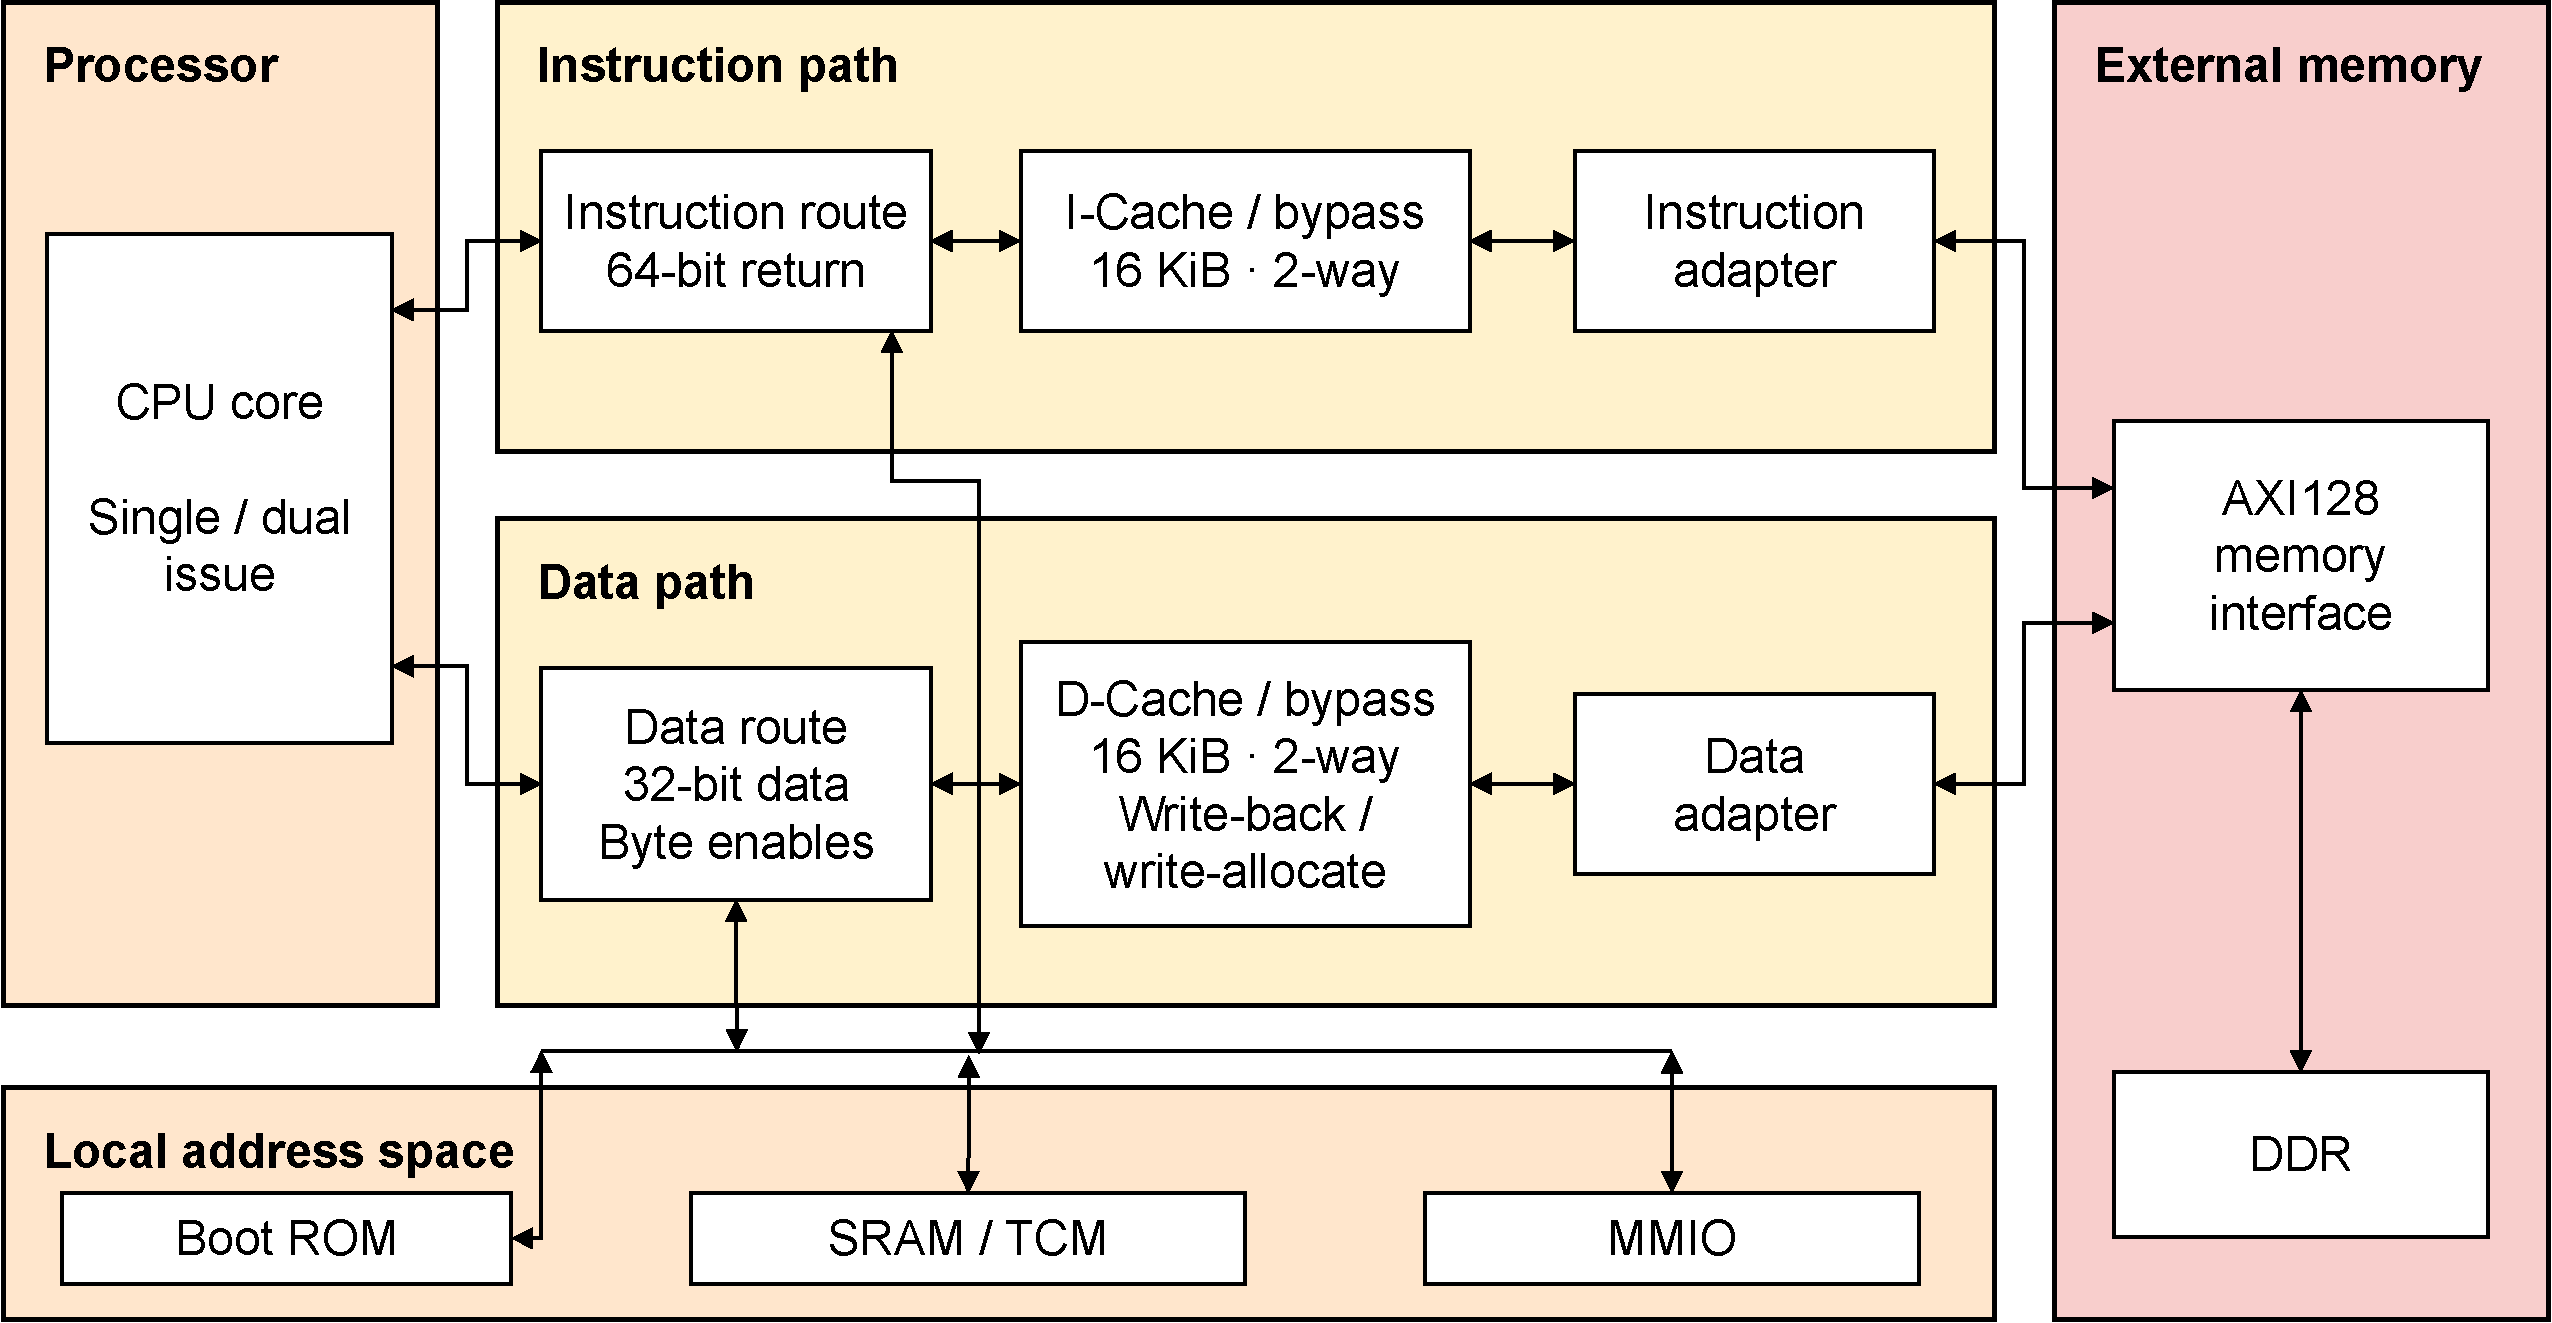
\includegraphics[width=\linewidth]{../figure/rv32-soc-page7.pdf}
\caption{CPU指令、数据与本地及外部存储接口}\label{fig:cpu-memory-interfaces}
\end{figure}


I-Cache和D-Cache各为16\,KiB，采用两路组相联、256组和32\,B缓存行，数据阵列使用同步RAM。
32\,bit地址划分为19\,bit标签、8\,bit组索引和5\,bit行内偏移。查询根据组索引读取两路标签及数据，标签匹配且有效时命中，否则选择替换行并启动填充。
替换控制使用全局交替状态选择路，D-Cache在目标组存在无效行时优先使用无效路。
下级DDR读通路以128\,bit返回数据，一条缓存行由两个16\,B数据拍组成。填充控制接收完整且无错误的响应后才建立有效缓存行；失败填充保持新行无效，并向原访问返回错误。
I-Cache从命中行中选择64\,bit取指包，D-Cache向加载存储单元提供32\,bit数据。

D-Cache采用写回、写分配策略。存储命中时按字节使能更新行内数据并设置脏位，完成响应由缓存内部产生。
存储未命中时，先处理被替换行，再读入目标缓存行，合并本次写数据并标记为脏行；后续对同一行的多次存储可在片上合并。
加载命中从数据阵列取得选中字，成功的可缓存加载响应可与满足条件的下一请求接纳重叠，返回数据通过寄存保持。
缓存未命中、维护操作和错误处理由阻塞式状态机串行完成。

替换脏行时，控制器将32\,B行拆为8个32\,bit字，逐字通过下级写通路提交，并等待各字的成功响应。
只有8个字全部写回成功，才清除原行脏状态并继续替换或维护。任一写响应失败时，原行保持有效和脏状态，终止后续填充并上报错误。
重试以整行为单位重新写回，以覆盖错误发生前已经到达DDR的部分数据。

缓存维护操作控制私有缓存数据的写回与失效，具体语义见表\ref{tbl:cpu-cache-maintenance}。
其中“清理”表示将脏数据写回并保留缓存行，“丢弃”表示直接取消有效性，“清理并失效”表示先写回再取消有效性。
\texttt{0x7C1}至\texttt{0x7C3}位于机器模式自定义读写CSR区，用于专用缓存维护，避开标准PMP地址。
维护仅由寄存器形式的\texttt{CSRRW}触发；单行维护以源寄存器提供目标地址，按缓存行匹配。
这三个命令CSR读回零，其他CSR指令形式不产生缓存维护动作。\texttt{0x7C0}独立用于内部计时比较。

\begin{reporttable}
\begin{longtable}{@{}p{0.22\linewidth}p{0.34\linewidth}p{0.37\linewidth}@{}}
\caption{CPU缓存维护操作}\label{tbl:cpu-cache-maintenance}\\
\toprule
操作 & 功能 & 缓存侧完成条件 \\
\midrule
\endfirsthead
\caption[]{CPU缓存维护操作（续）}\\
\toprule
操作 & 功能 & 缓存侧完成条件 \\
\midrule
\endhead
\bottomrule
\endfoot
CSR \texttt{0x7C2} & 清理匹配的D-Cache行，保留有效性 & 脏行全部写响应成功；未命中或干净行无需写回 \\
CSR \texttt{0x7C3} & 丢弃匹配的D-Cache行，包括其中的脏数据 & 行失效完成，不产生写回 \\
CSR \texttt{0x7C1} & 遍历D-Cache全部组和路，清理并失效 & 全部处理完成，或在首个写回错误后产生缓存错误响应 \\
\texttt{FENCE.I} & 排空先前数据事务，清理并失效D-Cache，再请求I-Cache失效 & D-Cache维护成功且I-Cache失效请求脉冲结束后恢复数据接纳；可缓存取指等待I-Cache失效完成 \\
\end{longtable}
\end{reporttable}

表中前三项的完成和错误条件指缓存接口响应，\texttt{FENCE.I}一项列出后续访问的接纳条件。维护指令按CSR通路进入WB，维护事务由加载存储单元和缓存继续跟踪，指令到达WB不等同于脏行已经成功写回。
维护错误也不经普通加载存储指令的E2异常条件上报，软件接口应区分CSR指令完成与缓存事务结果。

CPU私有区用于程序、栈及内部工作数据，DMA使用的帧缓存、共享张量和模型数据放置在不可缓存共享区，不建立可缓存别名。
软件在共享区写入完成后执行\texttt{fence rw,rw}，再将缓冲区标记为就绪并移交使用权；读取方根据完成事件及所有权状态读取数据。
普通访问屏障用于约束访问顺序，脏数据写回由专用缓存维护负责。

\texttt{FENCE.I}属于Zifencei扩展\cite{riscv-unpriv-20260120}。该指令发起后，缓存控制暂时停止接纳新的DDR取指和数据请求，排空已接纳的数据事务，完成D-Cache清理失效后向I-Cache发送失效请求。
包含该指令的软件使用\texttt{rv32im\_zicsr\_zifencei}目标配置。
D-Cache维护成功且I-Cache失效请求脉冲结束后，数据通路恢复接纳；可缓存取指继续由I-Cache自身状态机阻塞，直到逐组失效完成。
该操作通过缓存侧接纳控制约束后续取指，不向核心提供独立的维护完成响应。
内部清理若遇到写回错误，缓存子系统锁存协议故障并停止接纳请求，SoC路由器将后续普通DDR访问转换为错误响应，交由协调复位恢复。
CPU、缓存及外部事务控制共同管理复位；需要保留私有脏数据的计划复位应先完成缓存清理，再开始新的缓存有效状态。

\subsection{中断和异常}

CPU在机器模式下处理异常和中断，机器CSR保存处理器状态、使能位、待决位及异常返回信息\cite{riscv-priv-20260120}，主要接口见表\ref{tbl:cpu-csr}。
CSR指令支持寄存器和立即数两种操作数形式，提供交换、按位置位和按位清位操作，各寄存器的可写字段按实现掩码更新。
CSR访问同时检查地址是否实现、地址编码要求的特权级及只读属性。
访问未实现地址、越权访问或写入只读CSR时产生非法指令异常；\texttt{mepc}保存该指令PC，\texttt{mtval}保存指令字。
\texttt{CSRRS}/\texttt{CSRRC}的源寄存器为\texttt{x0}，或相应立即数形式的立即数为零时只读不写，可用于读取只读计数器。
固定WARL字段与未实现地址分别处理：\texttt{misa}具有读写地址编码，写入不改变实现固定的ISA字段；缓存维护命令CSR则按前述约定读回零。

\begin{reporttable}
\begin{longtable}{@{}p{0.27\linewidth}p{0.22\linewidth}p{0.44\linewidth}@{}}
\caption{CPU主要CSR接口}\label{tbl:cpu-csr}\\
\toprule
寄存器 & 地址 & 功能 \\
\midrule
\endfirsthead
\caption[]{CPU主要CSR接口（续）}\\
\toprule
寄存器 & 地址 & 功能 \\
\midrule
\endhead
\bottomrule
\endfoot
\texttt{mstatus} & \texttt{0x300} & 中断使能及陷入、返回状态 \\
\texttt{misa} & \texttt{0x301} & 固定返回\texttt{0x40001100}，表示RV32IM \\
\texttt{mie}、\texttt{mip} & \texttt{0x304}、\texttt{0x344} & 机器中断使能及锁存的待决状态 \\
\texttt{mtvec} & \texttt{0x305} & 四字节对齐的机器异常、中断直接入口 \\
\texttt{mscratch} & \texttt{0x340} & 机器处理程序暂存数据 \\
\texttt{mepc} & \texttt{0x341} & 陷入时保存的返回PC \\
\texttt{mcause}、\texttt{mtval} & \texttt{0x342}、\texttt{0x343} & 事件原因及对应异常信息 \\
\texttt{cycle}、\texttt{time} & \texttt{0xC00}、\texttt{0xC01} & 读取同一周期计数器的低32位 \\
\texttt{timeh} & \texttt{0xC81} & 读取周期计数器的高32位 \\
内部计时比较 & \texttt{0x7C0} & 比较低32位周期值，写入后重新布防 \\
\texttt{mvendorid} & \texttt{0xF11} & 厂商标识，实现为只读零 \\
\texttt{marchid} & \texttt{0xF12} & 架构标识，实现为只读零 \\
\texttt{mimpid} & \texttt{0xF13} & 实现版本标识，实现为只读零 \\
\texttt{mhartid} & \texttt{0xF14} & 处理器编号，固定为0 \\
\end{longtable}
\end{reporttable}

CPU提供一根外部IRQ输入，接收核外中断请求并在\texttt{mip}中形成MEIP待决状态。
机器软件中断通过CSR操作设置MSIP；内置计时比较器在周期计数低32位等于\texttt{0x7C0}中的比较值时设置MTIP，单次触发后撤销布防。
下一次计时事件由软件写入新的比较值重新设置。外部事件与内部计时事件均使用锁存的待决位，处理程序在处置中断源后清除相应状态。

中断受\texttt{mstatus.MIE}全局使能和\texttt{mie}分项使能控制。
多个中断同时满足受理条件时，按机器外部中断、机器软件中断、机器计时中断的次序选择，即MEI $>$ MSI $>$ MTI，原因号分别为11、3和7。
中断在流水线允许推进且没有受抑制的在途操作时进入异常控制路径，抑制被接管指令的正常副作用，并将中断状态传递至WB异常处理边界。

同步异常包括非法指令、\texttt{ECALL}、\texttt{EBREAK}、指令访问错误、指令地址不对齐、加载或存储访问错误以及数据地址不对齐。
异常原因与指令PC随流水线传递。\texttt{mtval}在数据访问及数据对齐异常时记录有效地址，在非法指令时记录指令字；取指类异常记录异常PC，分支目标不对齐时记录分支指令PC。
中断、\texttt{ECALL}和\texttt{EBREAK}对应的\texttt{mtval}为零，软件结合\texttt{mcause}判断其含义。

陷入时，异常控制写入\texttt{mepc}、\texttt{mcause}和\texttt{mtval}，将原MIE保存到MPIE并清除MIE，然后将取指地址重定向至\texttt{mtvec}。
软件将\texttt{mtvec}配置为四字节对齐的统一入口，由处理程序根据原因寄存器分派事件。
\texttt{MRET}从\texttt{mepc}恢复PC，将MPIE恢复到MIE并置MPIE为1；程序继续在机器模式下运行。
异常返回前，处理程序完成现场恢复，并根据异常类型决定保留或调整返回地址。

周期计数器按CPU时钟逐拍递增，流水线暂停期间继续计时。软件读取64\,bit计数时依次读取高位、低位和高位，若两次高位不一致则重读，避免低位进位造成计时撕裂。
板级基准使用该计数接口计算运行时间，指令完成数和流水线事件则由验证环境独立统计。

